\documentclass[a4paper, 12pt]{article}

% packages
\usepackage{amssymb}
\usepackage[fleqn]{mathtools}
\usepackage{tikz}
\usepackage{enumerate}
\usepackage{bussproofs}
\usepackage{xcolor}
\usepackage[margin=1.3cm]{geometry}
\usepackage{logicproof}
\usepackage{diagbox}
\usepackage{listings}
\usepackage{graphicx}
\usepackage{lstautogobble}
\usepackage{hyperref}
\usepackage{multirow}
\usepackage{tipa}
\usepackage{pgfplots}

% tikz libraries
\usetikzlibrary{
    decorations.pathreplacing,
    arrows,
    shapes.gates.logic.US,
    circuits.logic.US,
    calc,
    automata,
    positioning,
    intersections
}

\pgfplotsset{compat=1.16}

\pgfmathdeclarefunction{gauss}{2}{%
  \pgfmathparse{1/(#2*sqrt(2*pi))*exp(-((x-#1)^2)/(2*#2^2))}%
}

\allowdisplaybreaks % allow environments to break
\setlength\parindent{0pt} % no indent

% shorthand for verbatim
% this clashes with logicproof, so maybe fix this at some point?
\catcode`~=\active
\def~#1~{\texttt{#1}}

% code listing
\lstdefinestyle{main}{
    numberstyle=\tiny,
    breaklines=true,
    showspaces=false,
    showstringspaces=false,
    tabsize=2,
    numbers=left,
    basicstyle=\ttfamily,
    columns=fixed,
    fontadjust=true,
    basewidth=0.5em,
    autogobble,
    xleftmargin=3.0ex,
    mathescape=true
}
\newcommand{\dollar}{\mbox{\textdollar}} %
\lstset{style=main}

% augmented matrix
\makeatletter
\renewcommand*\env@matrix[1][*\c@MaxMatrixCols c]{%
\hskip -\arraycolsep
\let\@ifnextchar\new@ifnextchar
\array{#1}}
\makeatother

% ceiling / floor
\DeclarePairedDelimiter{\ceil}{\lceil}{\rceil}
\DeclarePairedDelimiter{\floor}{\lfloor}{\rfloor}

% custom commands
\newcommand{\indefint}[2]{\int #1 \, \mathrm{d}#2}
\newcommand{\defint}[4]{\int_{#1}^{#2} #3 \, \mathrm{d}#4}
\newcommand{\pdif}[2]{\frac{\partial #1}{\partial #2}}
\newcommand{\dif}[2]{\frac{\mathrm{d}#1}{\mathrm{d}#2}}
\newcommand{\limit}[2]{\raisebox{0.5ex}{\scalebox{0.8}{$\displaystyle{\lim_{#1 \to #2}}$}}}
\newcommand{\summation}[2]{\sum\limits_{#1}^{#2}}
\newcommand{\product}[2]{\prod\limits_{#1}^{#2}}
\newcommand{\intbracket}[3]{\left[#3\right]_{#1}^{#2}}
\newcommand{\laplace}{\mathcal{L}}
\newcommand{\fourier}{\mathcal{F}}
\newcommand{\mat}[1]{\boldsymbol{#1}}
\renewcommand{\vec}[1]{\boldsymbol{#1}}
\newcommand{\rowt}[1]{\begin{bmatrix}
    #1
\end{bmatrix}^\top}
\DeclareMathOperator*{\argmax}{argmax}
\DeclareMathOperator*{\argmin}{argmin}

\newcommand{\ulsmash}[1]{\underline{\smash{#1}}}

\newcommand{\powerset}[0]{\wp}
\renewcommand{\emptyset}[0]{\varnothing}

\makeatletter
\newsavebox{\@brx}
\newcommand{\llangle}[1][]{\savebox{\@brx}{\(\m@th{#1\langle}\)}%
  \mathopen{\copy\@brx\kern-0.5\wd\@brx\usebox{\@brx}}}
\newcommand{\rrangle}[1][]{\savebox{\@brx}{\(\m@th{#1\rangle}\)}%
  \mathclose{\copy\@brx\kern-0.5\wd\@brx\usebox{\@brx}}}
\makeatother
\newcommand{\lla}{\llangle}
\newcommand{\rra}{\rrangle}
\newcommand{\la}{\langle}
\newcommand{\ra}{\rangle}
\newcommand{\crnr}[1]{\text{\textopencorner} #1 \text{\textcorner}}
\newcommand{\bnfsep}[0]{\ |\ }
\newcommand{\concsep}[0]{\ ||\ }

\newcommand{\axiom}[1]{\AxiomC{#1}}
\newcommand{\unary}[1]{\UnaryInfC{#1}}
\newcommand{\binary}[1]{\BinaryInfC{#1}}
\newcommand{\trinary}[1]{\TrinaryInfC{#1}}
\newcommand{\quaternary}[1]{\QuaternaryInfC{#1}}
\newcommand{\quinary}[1]{\QuinaryInfC{#1}}
\newcommand{\dproof}[0]{\DisplayProof}

\newcommand{\ttbs}{\char`\\}
\newcommand{\lrbt}[0]{\ \bullet\ }

% colours
\newcommand{\violet}[1]{\textcolor{violet}{#1}}
\newcommand{\blue}[1]{\textcolor{blue}{#1}}
\newcommand{\red}[1]{\textcolor{red}{#1}}
\newcommand{\teal}[1]{\textcolor{teal}{#1}}

% reasoning proofs
\usepackage{ltablex}
\usepackage{environ}
\keepXColumns
\NewEnviron{reasoning}{
    \begin{tabularx}{\textwidth}{rlX}
        \BODY
    \end{tabularx}
}
\newcommand{\proofline}[3]{$(#1)$ & $#2$ & \hfill #3 \smallskip \\}
\newcommand{\proofarbitrary}[1]{& take arbitrary $#1$ \smallskip \\}
\newcommand{\prooftext}[1]{\multicolumn{3}{l}{#1} \smallskip \\}
\newcommand{\proofmath}[3]{$#1$ & = $#2$ & \hfill #3 \smallskip \\}
\newcommand{\prooftherefore}[1]{& $\therefore #1$ \smallskip \\}
\newcommand{\proofbc}[0]{\prooftext{\textbf{Base Case}}}
\newcommand{\proofis}[0]{\prooftext{\textbf{Inductive Step}}}

% ER diagrams
\newcommand{\nattribute}[4]{
    \node[draw, state, inner sep=0cm, minimum size=0.2cm, label=#3:{#4}] (#1) at (#2) {};
}
\newcommand{\mattribute}[4]{
    \node[draw, state, accepting, inner sep=0cm, minimum size=0.2cm, label=#3:{#4}] (#1) at (#2) {};
}
\newcommand{\dattribute}[4]{
    \node[draw, state, dashed, inner sep=0cm, minimum size=0.2cm, label=#3:{#4}] (#1) at (#2) {};
}
\newcommand{\entity}[3]{
    \node[] (#1-c) at (#2) {#3};
    \node[inner sep=0cm] (#1-l) at ($(#1-c) + (-1, 0)$) {};
    \node[inner sep=0cm] (#1-r) at ($(#1-c) + (1, 0)$) {};
    \node[inner sep=0cm] (#1-u) at ($(#1-c) + (0, 0.5)$) {};
    \node[inner sep=0cm] (#1-d) at ($(#1-c) + (0, -0.5)$) {};
    \draw
    ($(#1-c) + (-1, 0.5)$) -- ($(#1-c) + (1, 0.5)$) -- ($(#1-c) + (1, -0.5)$) -- ($(#1-c) + (-1, -0.5)$) -- cycle;
}
\newcommand{\relationship}[3]{
    \node[] (#1-c) at (#2) {#3};
    \node[inner sep=0cm] (#1-l) at ($(#1-c) + (-1, 0)$) {};
    \node[inner sep=0cm] (#1-r) at ($(#1-c) + (1, 0)$) {};
    \node[inner sep=0cm] (#1-u) at ($(#1-c) + (0, 1)$) {};
    \node[inner sep=0cm] (#1-d) at ($(#1-c) + (0, -1)$) {};
    \draw
    ($(#1-c) + (-1, 0)$) -- ($(#1-c) + (0, 1)$) -- ($(#1-c) + (1, 0)$) -- ($(#1-c) + (0, -1)$) -- cycle;
}

% actual document
\begin{document}
    \section*{CO212 - Networks and Communications}
        \subsection*{14th January 2020 \hfill Week 1, Lecture 1}
            \subsubsection*{Evolution of the Internet}
                Literally only writing this part so I have something for the first lecture.
                \begin{itemize}
                    \itemsep0em
                    \item (1969 - October) first message sent on ARPANET; "login", crashed after "l" and "o" were sent
                    \item (1971) universities in West and East coast of USA connected
                    \item (1980) London connected
                \end{itemize}
        \subsection*{14th January 2020 \hfill Week 2, Lecture 1}
            \subsubsection*{World Wide Web (WWW)}
                This is an example of an \textbf{application} on the internet, based on HTTP (HyperText Transfer Protocol).
                A web browser (the client) sends a \violet{request} to the web server over a pipe, which can be any form of connection between the two devices (can also be the same device), which in turn sends back a \teal{response}.
                \begin{center}
                    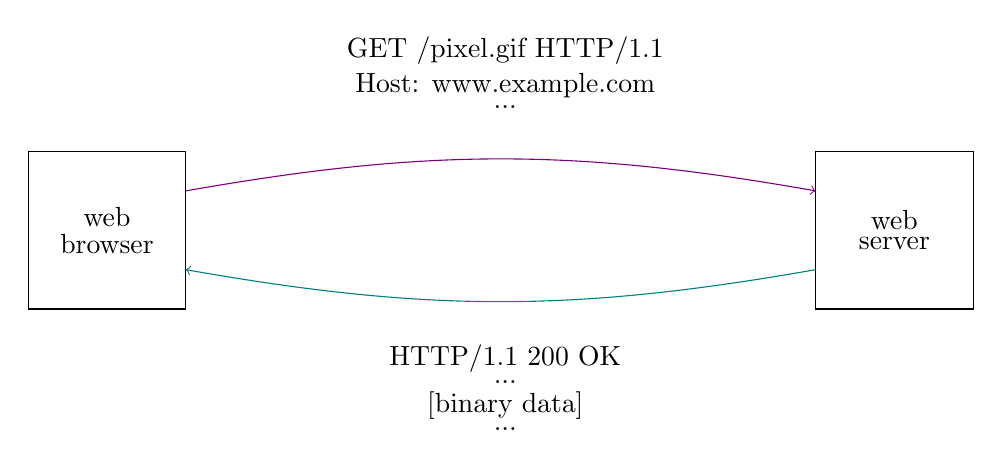
\begin{tikzpicture}
                        \node at (6, 1) {\shortstack{~GET /pixel.gif HTTP/1.1~\\~Host: www.example.com~\\~...~}};
                        \node at (6, -3) {\shortstack{~HTTP/1.1 200 OK~\\~...~\\~[binary data]~\\~...~}};
                        \node at (1, -1) {\shortstack{web\\browser}};
                        \node at (11, -1) {\shortstack{web\\server}};
                        \draw (0, 0) -- (2, 0) -- (2, -2) -- (0, -2) -- cycle;
                        \draw (10, 0) -- (12, 0) -- (12, -2) -- (10, -2) -- cycle;
                        \draw[violet] (2, -0.5) edge[->, bend left=10] (10, -0.5);
                        \draw[teal] (10, -1.5) edge[->, bend left=10] (2, -1.5);
                    \end{tikzpicture}
                \end{center}
            \subsubsection*{Layers}
                \begin{itemize}
                    \itemsep0em
                    \item \textbf{application layer}
                        \medskip

                        Any software written for the internet is on the application layer.
                    \item \textbf{transport layer}
                        \medskip

                        In the \textbf{transport layer}, packets leave your (client) machine to the server, and the server sends back packets to your client.
                        This layer divides a (big) message into smaller chunks, and sends them to the other side (re-ordered) to be presented to the recipient.
                    \item \textbf{network layer}
                        \medskip

                        The \textbf{route / path} (sequences of switches a packet goes through) each packet takes can be different from the others, and is often the most optimal route available.
                        This is done on the \textbf{network layer}, which routers are a part of.
                        \begin{center}
                            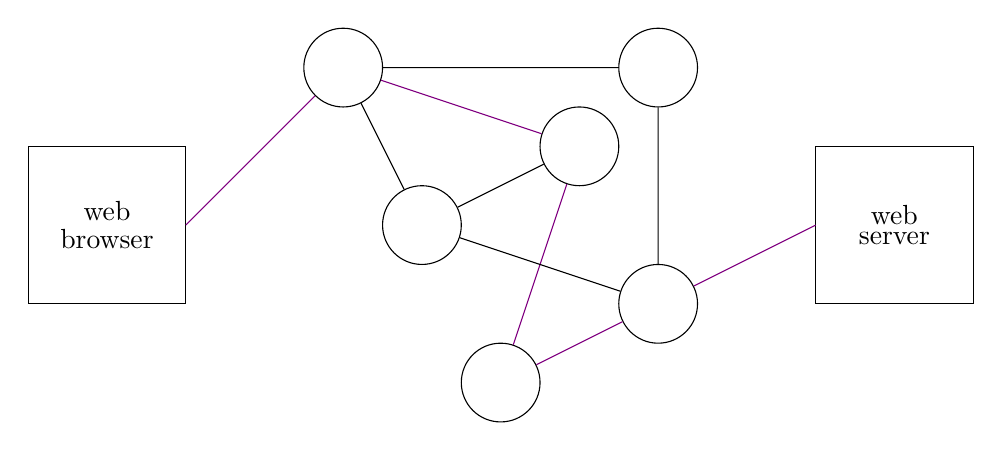
\begin{tikzpicture}
                                \node at (1, -1) {\shortstack{web\\browser}};
                                \node at (11, -1) {\shortstack{web\\server}};
                                \draw (0, 0) -- (2, 0) -- (2, -2) -- (0, -2) -- cycle;
                                \draw (10, 0) -- (12, 0) -- (12, -2) -- (10, -2) -- cycle;
                                \node[state, minimum size=1cm] (0) at (4, 1) {};
                                \node[state, minimum size=1cm] (1) at (5, -1) {};
                                \node[state, minimum size=1cm] (2) at (6, -3) {};
                                \node[state, minimum size=1cm] (3) at (7, 0) {};
                                \node[state, minimum size=1cm] (4) at (8, -2) {};
                                \node[state, minimum size=1cm] (5) at (8, 1) {};
                                \draw[violet] (2, -1) -- (0) -- (3) -- (2) -- (4) -- (10, -1);
                                \draw
                                (0) -- (1)
                                (0) -- (5)
                                (1) -- (3)
                                (1) -- (4)
                                (4) -- (5);
                            \end{tikzpicture}
                        \end{center}
                    \item \textbf{data link layer}
                        \medskip

                        Our devices are linked to the network on the \textbf{data link layer}, via network interface controllers (NICs).
                        Examples of this include Ethernet, fiber optic network cards, as well as wireless devices such as WiFi access points, and USB dongles for 4G.
                        A communication link is any connection between packet switches and / or end systems.
                    \item \textbf{physical layer}
                        \medskip

                        Finally, on the \textbf{physical layer}, there are various forms of communication media, including fiber-optic cables, twisted-pair copper wire, coaxial cables, and wireless local-area links (802.11, Bluetooth, etc).
                \end{itemize}
        \subsection*{16th January 2020 \hfill Week 2, Lecture 2}
            \subsubsection*{Circuit Switching}
                Old phones used circuit switching, which creates a connection between the two points, which is used for the entire communication.
                This isn't used for the internet as the failure of one node in the circuit would lead the the entire communication dropping - whereas a different route would be calculated in packet switching.
                \medskip

                Compared to packet switching, it has an expensive setup phase, but will need very little processing once the connection is established.
                However, it is inefficient for sharing resources - if a node is used as part of a circuit, it cannot be used by another connection for a different circuit.
                The resources are blocked once a connection is established (hence it is an inefficient way to use the network).
                On the other hand, packet switching has no setup cost, but has a processing cost, as well as space overhead, for every packet.
                It has a processing cost for forwarding the packets, as well as space overhead as there must be redundant data for each packet, such that it is self contained.
                It is specifically designed to share links, hence it allows for a better utilisation of network resources.
            \subsubsection*{Protocols}
                A protocol is a set of rules (an agreement between communicating parties on how communication is to proceed), run by end systems as well as packet switches.
                It must be unambiguous, complete (includes actions and / or responses for all possible situations), and also define all necessary message formats.
                The phases are as follows;
                \begin{itemize}
                    \itemsep0em
                    \item \textbf{handshake} \hfill establishes identities and / or context
                    \item \textbf{conversation} \hfill free-form exchange
                    \item \textbf{closing} \hfill terminating the conversation
                \end{itemize}
                The internet protocol stack is based on the 5 layers briefly covered in the previous lecture.
                Some examples of design issues that can be encountered are as follows;
                \begin{itemize}
                    \itemsep0em
                    \item \textbf{addressing} \hfill how to denote the intended recipient
                    \item \textbf{error control} \hfill how to detect (and possibly fix) transmission errors, e.g. checksums
                    \item \textbf{flow control} \hfill ensure data travels through communication media without issues
                    \item \textbf{multiplexing / demultiplexing} \hfill conversion of data into binary, and parallel communications
                    \item \textbf{routing} \hfill which route is chosen
                \end{itemize}
                Most network layers are either connection-oriented, where a connection is first established, data is exchanged, and the connection is finally released, or connectionless, where data is marked with its destination.
                \medskip

                The TCP/IP (4 layer) stack consists of application, transport, internet, and network access (which combines data link and physical).
                On the other hand, the OSI (7 layer) model consists of the application layer, presentation, session, transport, network, data link, and physical.
                \begin{center}
                    \hfill
                    \begin{tabular}{|c|}
                        \hline
                        \violet{application} \\
                        \hline
                        \violet{presentation} \\
                        \hline
                        \violet{session} \\
                        \hline
                        \blue{transport} \\
                        \hline
                        \red{network} \\
                        \hline
                        \teal{data link} \\
                        \hline
                        \teal{physical} \\
                        \hline
                    \end{tabular}
                    \hfill
                    \begin{tabular}{|c|}
                        \hline
                        \violet{application} \\
                        \hline
                        \blue{transport} \\
                        \hline
                        \red{network / internet} \\
                        \hline
                        \teal{data link} \\
                        \hline
                        \teal{physical} \\
                        \hline
                    \end{tabular}
                    \hfill
                    \begin{tabular}{|c|}
                        \hline
                        \violet{application} \\
                        \hline
                        \blue{transport} \\
                        \hline
                        \red{internet} \\
                        \hline
                        \teal{network access} \\
                        \hline
                    \end{tabular}
                    \hfill \phantom{}
                \end{center}
                A \textbf{service} is a set of primitives that a layer provides to the layer above it, whereas a \textbf{protocol} is a set of rules that prescribe the layout and meaning of packets.
                In a protocol stack, layer $k$ puts its entire packet as data into a layer $k - 1$ packet, the latter may add a header and / or a trailer.
                This may have to be split across several lower level packets (\textbf{fragmentation}).
                An example of protocol layering is as follows;
                \begin{center}
                    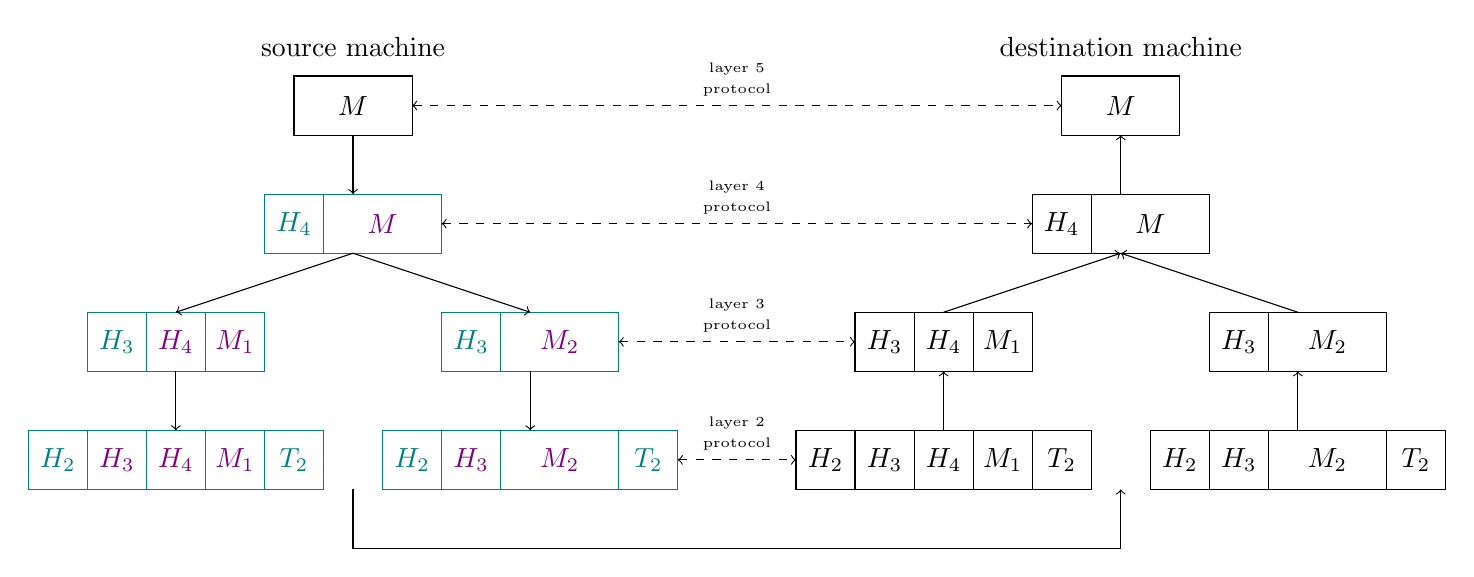
\begin{tikzpicture}[x=0.75cm, y=0.75cm]
                        \begin{scope}[shift={(0, 0)}]
                            \node at (1, 0.5) {source machine};
                            \node at (1, -0.5) {$M$};
                            \node at (0, -2.5) {\teal{$H_4$}};
                            \node at (1.5, -2.5) {\violet{$M$}};
                            \node at (-3, -4.5) {\teal{$H_3$}};
                            \node at (-2, -4.5) {\violet{$H_4$}};
                            \node at (-1, -4.5) {\violet{$M_1$}};
                            \node at (3, -4.5) {\teal{$H_3$}};
                            \node at (4.5, -4.5) {\violet{$M_2$}};
                            \node at (-4, -6.5) {\teal{$H_2$}};
                            \node at (-3, -6.5) {\violet{$H_3$}};
                            \node at (-2, -6.5) {\violet{$H_4$}};
                            \node at (-1, -6.5) {\violet{$M_1$}};
                            \node at (0, -6.5) {\teal{$T_2$}};
                            \node at (2, -6.5) {\teal{$H_2$}};
                            \node at (3, -6.5) {\violet{$H_3$}};
                            \node at (4.5, -6.5) {\violet{$M_2$}};
                            \node at (6, -6.5) {\teal{$T_2$}};
                            \draw (0, 0) -- (2, 0) -- (2, -1) -- (0, -1) -- cycle;
                            \draw[teal] (-0.5, -2) -- (2.5, -2) -- (2.5, -3) -- (-0.5, -3) -- cycle
                            (0.5, -2) -- (0.5, -3);
                            \draw[teal] (-3.5, -4) -- (-0.5, -4) -- (-0.5, -5) -- (-3.5, -5) -- cycle
                            (-2.5, -4) -- (-2.5, -5)
                            (-1.5, -4) -- (-1.5, -5);
                            \draw[teal] (2.5, -4) -- (5.5, -4) -- (5.5, -5) -- (2.5, -5) -- cycle
                            (3.5, -4) -- (3.5, -5);
                            \draw[teal] (-4.5, -6) -- (0.5, -6) -- (0.5, -7) -- (-4.5, -7) -- cycle
                            (-3.5, -6) -- (-3.5, -7)
                            (-2.5, -6) -- (-2.5, -7)
                            (-1.5, -6) -- (-1.5, -7)
                            (-0.5, -6) -- (-0.5, -7);
                            \draw[teal] (1.5, -6) -- (6.5, -6) -- (6.5, -7) -- (1.5, -7) -- cycle
                            (2.5, -6) -- (2.5, -7)
                            (3.5, -6) -- (3.5, -7)
                            (5.5, -6) -- (5.5, -7);
                            \draw
                            (1, -1) edge[->] (1, -2)
                            (1, -3) edge[->] (-2, -4)
                            (1, -3) edge[->] (4, -4)
                            (-2, -5) edge[->] (-2, -6)
                            (4, -5) edge[->] (4, -6);
                        \end{scope}
                        \draw[dashed]
                        (2, -0.5) edge[<->, above] node{\tiny\shortstack{layer 5\\protocol}} (13, -0.5)
                        (2.5, -2.5) edge[<->, above] node{\tiny\shortstack{layer 4\\protocol}} (12.5, -2.5)
                        (5.5, -4.5) edge[<->, above] node{\tiny\shortstack{layer 3\\protocol}} (9.5, -4.5)
                        (6.5, -6.5) edge[<->, above] node{\tiny\shortstack{layer 2\\protocol}} (8.5, -6.5);
                        \draw
                        (1, -7) -- (1, -8) -- (14, -8) edge[->] (14, -7);
                        \begin{scope}[shift={(13, 0)}]
                            \node at (1, 0.5) {destination machine};
                            \node at (1, -0.5) {$M$};
                            \node at (0, -2.5) {$H_4$};
                            \node at (1.5, -2.5) {$M$};
                            \node at (-3, -4.5) {$H_3$};
                            \node at (-2, -4.5) {$H_4$};
                            \node at (-1, -4.5) {$M_1$};
                            \node at (3, -4.5) {$H_3$};
                            \node at (4.5, -4.5) {$M_2$};
                            \node at (-4, -6.5) {$H_2$};
                            \node at (-3, -6.5) {$H_3$};
                            \node at (-2, -6.5) {$H_4$};
                            \node at (-1, -6.5) {$M_1$};
                            \node at (0, -6.5) {$T_2$};
                            \node at (2, -6.5) {$H_2$};
                            \node at (3, -6.5) {$H_3$};
                            \node at (4.5, -6.5) {$M_2$};
                            \node at (6, -6.5) {$T_2$};
                            \draw (0, 0) -- (2, 0) -- (2, -1) -- (0, -1) -- cycle;
                            \draw (-0.5, -2) -- (2.5, -2) -- (2.5, -3) -- (-0.5, -3) -- cycle
                            (0.5, -2) -- (0.5, -3);
                            \draw (-3.5, -4) -- (-0.5, -4) -- (-0.5, -5) -- (-3.5, -5) -- cycle
                            (-2.5, -4) -- (-2.5, -5)
                            (-1.5, -4) -- (-1.5, -5);
                            \draw (2.5, -4) -- (5.5, -4) -- (5.5, -5) -- (2.5, -5) -- cycle
                            (3.5, -4) -- (3.5, -5);
                            \draw (-4.5, -6) -- (0.5, -6) -- (0.5, -7) -- (-4.5, -7) -- cycle
                            (-3.5, -6) -- (-3.5, -7)
                            (-2.5, -6) -- (-2.5, -7)
                            (-1.5, -6) -- (-1.5, -7)
                            (-0.5, -6) -- (-0.5, -7);
                            \draw (1.5, -6) -- (6.5, -6) -- (6.5, -7) -- (1.5, -7) -- cycle
                            (2.5, -6) -- (2.5, -7)
                            (3.5, -6) -- (3.5, -7)
                            (5.5, -6) -- (5.5, -7);
                            \draw
                            (1, -1) edge[<-] (1, -2)
                            (1, -3) edge[<-] (-2, -4)
                            (1, -3) edge[<-] (4, -4)
                            (-2, -5) edge[<-] (-2, -6)
                            (4, -5) edge[<-] (4, -6);
                        \end{scope}
                    \end{tikzpicture}
                \end{center}
                Note that the connection between the two machines can have multiple nodes in between, that can read up to a different physical layer.
                For example, if there was a link-layer switch after the source machine, it can read up to the link layer (layer 2), remove and add headers / trailers, and then send it on to the next device.
                The next device may be a router for example, which can read up to the network layer (layer 3), and do the same.
                \medskip

                The data from the layer above is known as the \violet{SDU (service data unit)}, and the SDU combined with a header, added by the current layer, is known as the \teal{PDU (protocol data unit)}.
        \subsection*{16th January 2020 \hfill Week 2, Lecture 3}
            \subsubsection*{Protocol Layers}
                The types of protocols on each layer are as follows;
                \begin{itemize}
                    \itemsep0em
                    \item \textbf{application layer}
                        \medskip

                        Protocols on the application layer defines functionality and message formats.
                        Some examples are as follows;
                        \begin{itemize}
                            \itemsep0em
                            \item \textbf{traditional} \hfill name services (DNS), sending email (SMTP), file transfer (FTP), web (HTTP(S))
                            \item \textbf{modern}
                                \subitem includes middleware protocols to support distributed systems with special protocols to handle replication, fault tolerance, caching, etc.
                            \item \textbf{high-level} \hfill special application-level protocols for e-commerce, banking etc.
                            \item \textbf{peer-to-peer} \hfill BitTorrent, old-Skype (awful API)
                        \end{itemize}
                    \item \textbf{transport layer}
                        \medskip

                        These protocols generally offer connection-oriented (TCP) as well as connectionless (UDP) services, which have varying degrees of reliability.
                        These often provide a network interface to application via sockets.
                        It's also important to note there is a difference between reliability and security; the former guarantees that the data is sent, whereas the latter ensures that it is encrypted in some form.
                        This layer also provides flow control; mechanisms to ensure fast senders don't overwhelm slow receivers.
                    \item \textbf{network layer}
                        \medskip

                        In this layer, the protocols generally describe how routing is performed, such as determining which computers / routers are in the network, the best route between two points, how to handle faults (such as a device going down), as well as handling congestion (when a router is overloaded and packets are dropped).
                    \item \textbf{data link layer}
                        \medskip

                        In this layer, we need to detect bit transmission errors.
                        This can be done by adding redundancy bits in frames to detect errors - for example adding a parity bit to every 7 bits, where a 1 indicates an odd number of 1s, and a 0 indicates an even number of 1s, or adding a checksum (cyclic redundancy check) which should match the bits before it.
                        \medskip

                        It also specifies how many computers can share a common channel, with the medium access control sub-layer (MAC).
                        A well known protocol is the Ethernet protocol.
                    \item \textbf{physical layer}
                        \medskip

                        This describes the transmission of raw bits, in terms of the physical mechanical and electrical issues.
                        For example, when two computers are connected with a wire, -3V may indicate to a binary 1, and +4V may correspond to a binary 0.
                        It may also specify the number of times the voltage can be changed per second.
                        \medskip

                        For example if the voltage can be changed 20,000 times per second, it indicates that the maximum transfer rate is 20,000 bits per second, which is 20 Kbps (20 kilobits per second).
                \end{itemize}
            \subsubsection*{Units}
                \begin{itemize}
                    \itemsep0em
                    \item 1 Byte = 8 bits \hfill note that a byte has an uppercase B, whereas a bit has lowercase b
                    \item 1000 Bytes = 1 KB \hfill (Kilobyte)
                    \item 1024 Bytes = 1 KiB \hfill (Kibibyte)
                \end{itemize}
                Typically we use powers of 10 for networks, but as long as we are consistent in what we use it is fine.
            \subsubsection*{Quantifying Data Transfer}
                \begin{itemize}
                    \itemsep0em
                    \item \textbf{bandwidth}
                        \subitem the amount of information that \textbf{can} get into the connection in a time unit
                    \item \textbf{throughput}
                        \subitem the amount of information that \textbf{actually} get into the connection in a time unit - at steady-state, we assume zero accumulation of traffic therefore the input and output throughputs are equal
                    \item \textbf{latency}
                        \subitem the time it takes for one bit to go through the connection
                \end{itemize}
                Note that for the following formula, we use these values;
                \begin{itemize}
                    \itemsep0em
                    \item $t_0$ \hfill the time the first packet leaves the source
                    \item $t_1$ \hfill the time the first packet reaches the destination
                    \item $t_2$ \hfill the time all the packets reach the destination
                    \item $L$ \hfill the size of the packet in bits
                    \item latency (propagation delay) \hfill $d = t_1 - t_0$ (generally $\frac{\text{distance}}{\text{wave propagation speed}}$)
                        \subitem note that this is half the RTT (round-trip time)
                    \item throughput (link bandwidth) \hfill $R = \frac{L}{t_2 - t_1}$ (generally $\frac{\text{transferred bits}}{\text{duration}}$)
                    \item packetization (transmission delay / store-and-forward delay) \hfill $\frac{L}{R}$
                        \subitem time it takes for the entire packet to be received after the first bit is received
                    \item transfer time (propagation delay + transmission delay) \hfill $\Delta = d + \frac{L}{R}$
                \end{itemize}
                However, it's important to note that the connections are (almost) never direct, and therefore will have additional delays at each router.
                Note that our bandwidth is also bottlenecked by the lowest bandwidth.
                \begin{center}
                    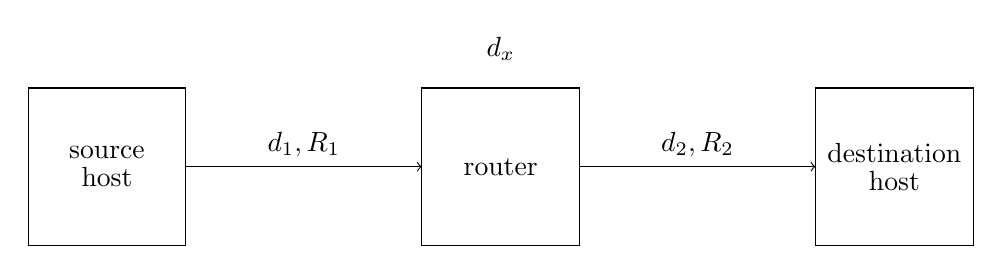
\begin{tikzpicture}
                        \node at (1, -1) {\shortstack{source\\host}};
                        \node at (6, 0.5) {$d_x$};
                        \node at (6, -1) {router};
                        \node at (11, -1) {\shortstack{destination\\host}};
                        \draw (0, 0) -- (2, 0) -- (2, -2) -- (0, -2) -- cycle;
                        \draw (5, 0) -- (7, 0) -- (7, -2) -- (5, -2) -- cycle;
                        \draw (10, 0) -- (12, 0) -- (12, -2) -- (10, -2) -- cycle;
                        \draw
                        (2, -1) edge[->, above] node{$d_1, R_1$} (5, -1)
                        (7, -1) edge[->, above] node{$d_2, R_2$} (10, -1);
                    \end{tikzpicture}
                \end{center}
                \begin{align*}
                    d_\text{end-end} & = \begin{cases}
                        d_1 + \frac{L}{R_1} + d_x + d_2 & R_1 < R_2 \\
                        d_1 + d_x + \frac{L}{R_2} + d_2 & R_1 \geq R_2
                    \end{cases} \\
                    & = d_1 + d_x + d_2 + \frac{L}{\min (R_1, R_2)}
                \end{align*}
                The router delay, $d_x$ has two components; the processing delay $d_\text{proc}$ which is the processing time (checking for bit errors and determining the output link), as well as $d_q$, which is the queueing delay - the time waiting at the output link for transmission, which depends on how congested the router is.
                We can quantify the \textbf{traffic intensity} as follows;
                \begin{align*}
                    R & = \text{link bandwidth} \\
                    L & = \text{packet length (bits)} \\
                    a & = \text{average packet arrival rate} \\
                    \frac{La}{R} & = \text{traffic intensity} \\
                    \frac{La}{R} & \approx 0 & \text{small average queueing delay} \\
                    \frac{La}{R} & \to 1 & \text{large average queueing delay} \\
                    \frac{La}{R} & > 1 & \text{more working arriving than can be serviced, infinite delay}
                \end{align*}
        \subsection*{21st January 2020 \hfill Week 3, Lecture 1}
            \subsubsection*{Clients and Servers}
                We can distinguish between the two roles in a pair of communicating processes, in a connection-oriented model;
                \begin{itemize}
                    \itemsep0em
                    \item \textbf{client} \hfill initiates communication
                    \item \textbf{server} \hfill waits to be contacted
                \end{itemize}
                On the other hand, some applications have processes that act as both the client and the server, which is referred to P2P (or peer-to-peer) architecture.
            \subsubsection*{End System Applications}
                Internet applications are processes on the end systems.
                They must have a way of addressing each other, either via the internet (such as chat servers), or they can directly communicate (such as FTP) - but this depends on the protocol in use.
                Note that a single end system (or host) can run multiple programs, which run multiple processes, all of which connect through a network API provided by the operating system.
                Each process is addressed within its host by a \textbf{port number}.
                When an application wants to communicate with another application, the OS opens a socket, which allows data to be transferred between the two machines.
                \begin{center}
                    \begin{minipage}[t]{0.485\textwidth}
                        client application
                        \begin{enumerate}[1.]
                            \itemsep0em
                            \item create a socket $C$ by connecting to server application (connecting to host $H$ on port $P$)
                            \item read and write data to socket $C$
                            \item disconnect and destroy $C$
                        \end{enumerate}
                    \end{minipage}
                    \hfill
                    \begin{minipage}[t]{0.485\textwidth}
                        server application (on host $H$)
                        \begin{enumerate}[1.]
                            \itemsep0em
                            \item create a socket $S$ by accepting connection on part $P$ (port is often called a server socket)
                            \item read and write data to socket $S$
                            \item disconnect and destroy $S$
                        \end{enumerate}
                    \end{minipage}
                \end{center}
                The server application can open more sockets to server multiple clients at a time.
                A DDoS (distributed denial of service) attack works by opening many sockets, preventing the server from serving legitimate requests.
            \subsubsection*{The World Wide Web}
                Invented in 1989 (formally defined in 1991) by Sir Tim Berners-Lee.
                Based on the idea of hypertext and hyperlinks (based on a proposal by William Tunnicliffe in late 1960s).
                Commonly used terminology is as follows;
                \begin{itemize}
                    \itemsep0em
                    \item \textbf{document} \hfill a webpage is called a document
                    \item \textbf{object} \hfill any called within a document (images, stylesheets, etc.)
                    \item \textbf{Uniform Resource Locator (URL)} \hfill specifies the address of an object
                    \item \textbf{browser} \hfill also called user agent - client used to access documents
                    \item \textbf{web server} \hfill application that makes documents and objects available through HTTP
                \end{itemize}
            \subsubsection*{Protocol}
                In general, the request and reply would include the following;
                \begin{center}
                    \begin{minipage}[t]{0.485\textwidth}
                        request
                        \begin{itemize}
                            \itemsep0em
                            \item protocol version
                            \item URL specification
                            \item connection attributes
                            \item content / feature negotiation
                        \end{itemize}
                    \end{minipage}
                    \hfill
                    \begin{minipage}[t]{0.485\textwidth}
                        reply
                        \begin{itemize}
                            \itemsep0em
                            \item protocol version
                            \item reply status / value
                            \item connection attributes
                            \item object attributes
                            \item content specification
                            \item content
                        \end{itemize}
                    \end{minipage}
                \end{center}
                A protocol should always include a version number, as it allows the protocol design to change.
                HTTP/2 will replace HTTP/1.x in the next few years (hopefully), as the former is able to fully multiplex a connection since all content is binary, and can use a single TCP connection for parallelism.
                \medskip

                The URL contains the host name, which determines where the requests goes, by mapping to a network address.
                The request consists of a request line, such as ~GET /path/to/index.html HTTP/1.1~, zero or more header lines, an empty line, followed by the object body (which can be empty).
                The request line contains a method, such as;
                \begin{itemize}
                    \itemsep0em
                    \item ~GET~ \hfill retrieve the object identified by the URL
                    \item ~POST~ \hfill allows for submission of data to the server
                    \item ~HEAD~ \hfill similar to ~GET~ but only receives headers
                    \item ~PUT~ \hfill requests the enclosed object to be stored under the given URL
                    \item ~DELETE~ \hfill deletes the given object
                    \item ~OPTIONS~ \hfill requests the available communication options for the given object
                \end{itemize}
                The status code in a server response is generally as follows;
                \begin{itemize}
                    \itemsep0em
                    \item ~1xx~ \hfill informational
                    \item ~2xx~ \hfill successful
                    \item ~3xx~ \hfill redirection (e.g. object has temporarily or permanently moved)
                    \item ~4xx~ \hfill client error (e.g. malformed request, unauthorised, object not found, method not allowed)
                    \item ~5xx~ \hfill server error (e.g. internal server error, service overloaded)
                \end{itemize}
        \subsection*{23rd January 2020 \hfill Week 3, Lecture 2}
            \subsubsection*{How HTTP uses TCP}
                HTTP uses TCP as it is essentially a file transfer protocol, which needs to be connection-oriented.
                The first version of HTTP uses a TCP connection for each object, which was an inefficient use of both the network and the operating system.
                HTTP/1.1 introduced persistent connection, which allows for an existing connection to be used to issue multiple requests (either sending a request, waiting for a response, sending the next request and so on, or through pipelining) - which will eventually close with a timeout.
                Pipelining allows the client to send all its requests without waiting for a response, and the server delivers them in response.
            \subsubsection*{Web Caching}
                A proxy is a server which acts as an intermediate between the client and the destination server.
                This can be used for caching by storing a copy of the content, which reduces load on the origin server, and also allows for lower latency.
                Data isn't cached for an extended period of time as it can lead to stale data (where old content is served to a user, even after the content is changed on the origin server).
                Proxies can also protect the clients by providing anonymity, as well blocking malicious content through the use of a single firewall on the proxy.
                However, this also acts as a single point of failure - if the proxy fails then the clients may not be able to connect.
                \medskip

                A ~HEAD~ request could be used to see if an object has been updated, which is less expensive than retrieving the entire object with a ~GET~ request.
                The request can also include ~Cache-Control: no-cache~, which indicates it does not want cached objects, thus requiring proxies to go to the origin server, or ~Cache-Control: max-age=20~, which only gets a cached object if the cache is less than 20 seconds old.
                \medskip

                On the other hand, the reply can also include ~Cache-Control: no-cache~, which informs the proxy not to cache the object, or ~Cache-Control: maxage=100; must-revalidate~, which specifies to the proxy that it must revalidate the object after 100 seconds.
            \subsubsection*{Sessions}
                Note that HTTP is a \textbf{stateless} protocol, which means that responses have no memory of past requests.
                However, HTTP allows higher-level applications to maintain \textbf{stateful} sessions, via the use of cookies.
                The ~Set-Cookie~ header is sent from a server, informing the client to store the cookie as a session identifier for that site.
                On the other hand, the client sends a ~Cookie~ header, which tells the server which session the request belongs to.
                This can be useful for storing identifying a user on a page (allowing for personalised pages).
                However, this can be also be used to track users for profiling and targeted advertising - leading to privacy issues.
            \subsubsection*{Dynamic Web Pages}
                Servers often generate pages on-the-fly, instead of only serving statically stored pages.
                CGI (common gateway interface) allows you to identify a program and its parameters in a URL, which then starts a process to execute the program and return any results as a regular web page.
                On the other hand, servelets in Java maintain state (whereas CGI is stateless), and the webserver contains an instance of the JVM.
                \medskip

                Another approach is for the web page to incorporate interpretable code, which is executed when the page is being processed on the client-side (via JavaScript).
                It's important to distinguish this from server-side processing in something such as PHP, which the user should not see.
            \subsubsection*{IP and Hosts}
                Each end system is identified and addressed by its IP address, which is 32 bits in IPv4, or 128 bits in IPv6.
                This is easy to process by a computer, as it can easily work in powers of two, but not practical for people to use.
                \medskip

                Host names are used to create human-readable "aliases" for IP addresses.
                Originally, before 1983, all mappings were in the ~hosts~ file, since there weren't many different hosts.
                However, as more hosts became present, DNS (Domain Name System) was developed, which provides a distributed lookup facility.
                \medskip

                There are 13 root DNS servers, which know where the top-level servers are located.
                The top-level domain servers are each associated with a top-level domain.
                However, knowing where to connect to requires a large amount of communication between servers.
                This can therefore be a bottleneck for applications, and also be a critical point of failure.
                To circumvent this, we can also cache DNS lookups.
                This improves performance as we do not have to do as much communication, and it also reduces the overall load on the DNS infrastructure.
                \medskip

                However, this can be an issue if enough DNS servers advertise an incorrect lookup, causing subsequent requests to point to an incorrect IP (DNS cache poisoning).
                \medskip

                DNS query types are as follows;
                \begin{itemize}
                    \itemsep0em
                    \item ~A~ \hfill maps a host name to its address, \textbf{name} is a host name, and \textbf{value} is its IP address
                    \item ~NS~
                        \subitem a query for a name server, \textbf{name} is a domain name, and \textbf{value} is the authoritative name server for that domain
                    \item ~CNAME~
                        \subitem a query for a canonical name, \textbf{name} is a host name alias, \textbf{value} is the primary host name
                    \item ~MX~
                        \subitem a query for the mail exchange server \textbf{name} is a host or domain name, and \textbf{value} is the name of the mail server handling incoming mail
                \end{itemize}
                The DNS protocol is connectionless, and runs on UDP port 53.
                UDP (best effort) is used since it only involves two network packets (request and response), setting up and closing a TCP (reliable) connection every time would be wasteful.
                If it fails, it can just try again.
                \medskip

                \textbf{Round Robin DNS} is a load balancing technique, as it responds to DNS requests with a list of IP addresses instead of a single IP address.
                The IP at the top of list is returned a set number of times before it is moved to the bottom of the list (the IP that was previously second in the list is now at the top).
                If load balancing is used, the TTL should be small, as we want this to constantly change depending on server load.
        \subsection*{23rd January 2020 \hfill Week 3, Lecture 3}
            \subsubsection*{Content Distribution Networks (CDNs)}
                We have the following options when we want to provide a streaming service from millions of videos to many simultaneous users;
                \begin{enumerate}[1.]
                    \itemsep0em
                    \item single, large "mega-server"
                        \begin{itemize}
                            \itemsep0em
                            \item single point of failure, and point of network congestion
                            \item long path to distant clients (slow)
                            \item multiple copies of video sent over outgoing link
                        \end{itemize}
                        This solution does not scale to a large amount of users.
                    \item store multiple copies of videos at multiple geographically distributed sites
                        \begin{itemize}
                            \itemsep0em
                            \item \textbf{enter deep} \hfill push CDN servers into many access networks (close to users)
                                \subitem used by Akamai (216000+ servers, 120+ countries, 1500+ networks)
                            \item \textbf{bring home} \hfill smaller number of large clusters in PoPs near (not within) access networks
                                \subitem used by Limelight (80+ PoPs - Points of Presence)
                        \end{itemize}
                \end{enumerate}
                A CDN DNS can select a good CDN node by picking the CDN node closest to  the client, or a CDN node with the shortest delay to the client.
                However, it's important to note that the CDN doesn't know the IP address of the client, only the address of the local DNS which may not be fully accurate.
                An alternative is to let the client decide by giving a list of CDN servers.
                The client can then select the "best" based on the lowest RTT.
            \subsubsection*{Electronic Mail}
                While email was able to achieve asynchronous communication, one-to-many communication, as well as multimedia content it had a number of limitations.
                Privacy and security was an issue, as there was initially no authentication - hence messages could be modified or forged, and messages could be read by others.
                Additionally, it was unreliable as there were no delivery guarantees, and had no reliable acknowledgement system.
                \begin{center}
                    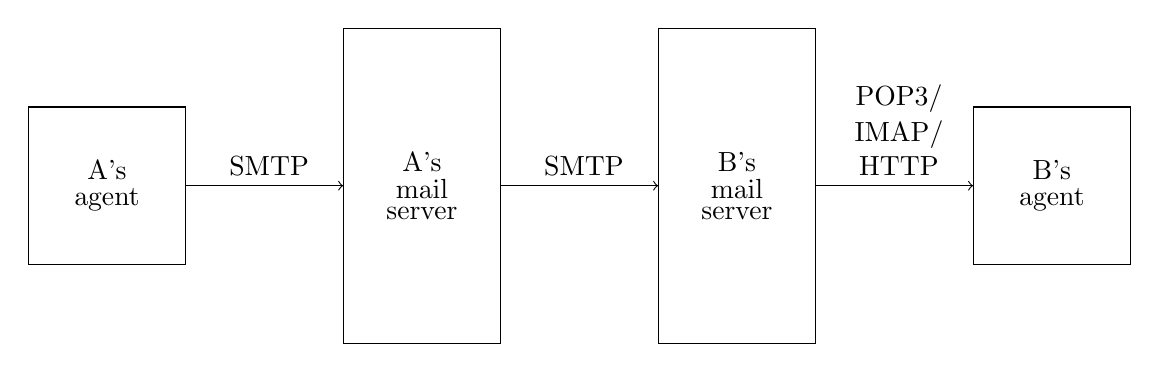
\begin{tikzpicture}
                        \node at (1, -1) {\shortstack{A's\\agent}};
                        \node at (5, -1) {\shortstack{A's\\mail\\server}};
                        \node at (9, -1) {\shortstack{B's\\mail\\server}};
                        \node at (13, -1) {\shortstack{B's\\agent}};
                        \draw (0, 0) -- (2, 0) -- (2, -2) -- (0, -2) -- cycle;
                        \draw (4, 1) -- (6, 1) -- (6, -3) -- (4, -3) -- cycle;
                        \draw (8, 1) -- (10, 1) -- (10, -3) -- (8, -3) -- cycle;
                        \draw (12, 0) -- (14, 0) -- (14, -2) -- (12, -2) -- cycle;
                        \draw
                        (2, -1) edge[->, above] node{~SMTP~} (4, -1)
                        (6, -1) edge[->, above] node{~SMTP~} (8, -1)
                        (10, -1) edge[->, above] node{\shortstack{~POP3/~\\~IMAP/~\\~HTTP~}} (12, -1);
                    \end{tikzpicture}
                \end{center}
                The user agent is the client the user uses to read, compose, reply, send and forward messages.
                The mail server can do the following;
                \begin{itemize}
                    \itemsep0em
                    \item accept messages for remote delivery (delivers message to remote destination server with transport protocol)
                    \item accept messages for local delivery (saves messages in local persistent mailbox)
                    \item allows user agents to access local mailboxes (to allow for retrieval and / or deletion of messages)
                \end{itemize}
            \subsubsection*{Simple Mail Transfer Protocol}
                It's important to note that the 'S' in SMTP does not stand for secure (no authentication).
                This is a connection-oriented protocol (TCP), on port 25.
                As it is a very simple protocol, it can be left unsecured - this is often targeted by spammers and phishers who use unsecured mail servers to send mail without using their own resources.
                \medskip

                The general format of using SMTP is headers, followed by an empty line, and then content.
                A single dot is used to end the email, and ~QUIT~ is used to exit.
                SMTP is completely oblivious to the contents of a message, other than the \textbf{received} header, which is added by each receiving SMTP server.
                This can be used to trace the origins of an email.
                \medskip

                The initial message format had many limitations - it only supported 7-bit text content, and was essentially only usable for the English language.
                The MIME (multipurpose internet mail extensions) format defined useful extensions on top of SMTP, which includes the following types;
                \begin{itemize}
                    \itemsep0em
                    \item ~text/plain~ \hfill normal ASCII message
                    \item ~text/html~ \hfill HTML-formatted message
                    \item ~image/jpeg~ \hfill contains only an image file
                    \item ~multipart/mixed~ \hfill consists of multiple parts
                \end{itemize}
            \subsubsection*{Post Office Protocol (POP3) and IMAP}
                The user's mailbox is often stored on a different machine than the user agent, but we need remote access to incoming (and outgoing) messages.
                However, POP3 is insecure (at least on port 110), due to the transmission of credentials in plain text.
                It also implicitly assumes the retrieved mail is deleted at the server, which isn't useful if people wanted to access mail from different clients.
                \medskip

                The internet message access protocol (IMAP) solves this, by storing messages on a server, and requiring the client to be online to read mail.
            \subsubsection*{Dark Web}
                TOR (The Onion Router) hides the user behind a series of machines (proxies), and also allows for access to ~.onion~ sites (as well as regular ones).
                This can be used for privacy purposes, as well as for circumventing censorship.
                The exit nodes of TOR can be owned by law enforcement agencies, allowing for a user to be compromised if they were to subpoena all intermediate proxies.
                \medskip

                Not that this shouldn't be confused with the \textbf{deep web}, which is typically just not indexed on the surface web.
        \subsection*{27th January 2020 \hfill Week 4, Lecture 1}
            \subsubsection*{Transport Layer}
                The transport layer provides both reliable connection-oriented services (TCP - transmission control protocol), as well as unreliable connection-less services (UDP - user datagram protocol).
                This provides for logical communication between application processes, and only runs on end hosts (not routers / switches).
                TCP data are called segments, whereas UDP data are called datagrams.
                \medskip

                We also assume that the underlying layer is working, with every host having a unique IP address, and that IP is a "best-effort" delivery service.
                This means that it has no guarantees on the integrity of data (or packet) transmission, nor does it guarantee the order of delivery of packets or segments.
            \subsubsection*{Data Encapsulation}
                For each layer, we have the following terminology - we can't refer to everything as packets;
                \begin{itemize}
                    \itemsep0em
                    \item application layer \hfill data
                    \item transport layer \hfill TCP segments or UDP datagrams
                        \subitem (TCP only) segmentation can be done when the segments are too large - if the UDP datagrams are too large, it cannot be sent
                    \item network / internet layer \hfill IP datagrams (or packets)
                        \subitem similarly, fragmentation can be done when the packets are too large
                    \item data link layer \hfill frames
                    \item physical layer \hfill bits
                \end{itemize}
            \subsubsection*{Ports}
                Note that it's possible for a client (one IP) to communicate with the same host (one IP) via multiple applications, such as HTTP and SMTP.
                Each application on ta host is identified with a unique port number - they can be thought of as cross-platform process identifiers.
                A socket consists of two pairs of ~ip\_address~ + ~port\_number~ + ~TCP/UDP~;
                such as
                \begin{center}
                    ~146.179.40.24:80 TCP~ $\Leftrightarrow$ ~192.168.1.1:7155 TCP~
                \end{center}
                The first 1024 ports (0 - 1023) are reserved, and cannot be used to form a connection as a client (unless it is done as a superuser).
            \subsubsection*{Transmission Control Protocol}
                TCP is the Internet's primary transport protocol.
                It is a connection-oriented service, and endpoints initially perform a handshake to establish a connection.
                This is a full-duplex service, thus both endpoints can send a receive at the same time.
                Some definitions for TCP are as follows;
                \begin{itemize}
                    \itemsep0em
                    \item \textbf{TCP segment} \hfill "envelope" for TCP data
                    \item \textbf{maximum segment size (MSS)}
                        \subitem maximum amount of application data transmitted in a single segment (does not include headers) - typically related to MTU to avoid network-level fragmentation
                    \item \textbf{maximum transmission unit (MTU)} \hfill largest link-layer frame available to the sender host
                        \subitem path MTU discovery (PMTUD) is used to determine the largest link-layer frame that can be sent on all links from the sender to the receiver
                \end{itemize}
                The TCP header consists of the following fields;
                \begin{itemize}
                    \itemsep0em
                    \item \violet{source and destination ports} \hfill 16-bit each (identifies applications)
                    \item \violet{sequence number} \hfill 32-bit (used to implement reliable data transfer)
                        \medskip

                        These numbers are not associated with the segments, but instead are associated with the bytes in the data stream.
                        It indicates the sequence number (the place) of the first byte carried by the TCP segment.
                        When the connection is initialised, a random ISN (initial sequence number) is decided upon to avoid accidentally receiving leftover segments.
                    \item \violet{acknowledgement number} \hfill 32-bit (used to implement reliable data transfer)
                        \medskip

                        Represents the first number not yet seen by the receiver (one higher than the sequence number of the last bit received).
                        These can be cumulative, and typically TCP implementations acknowledge every other packet;
                        \begin{center}
                            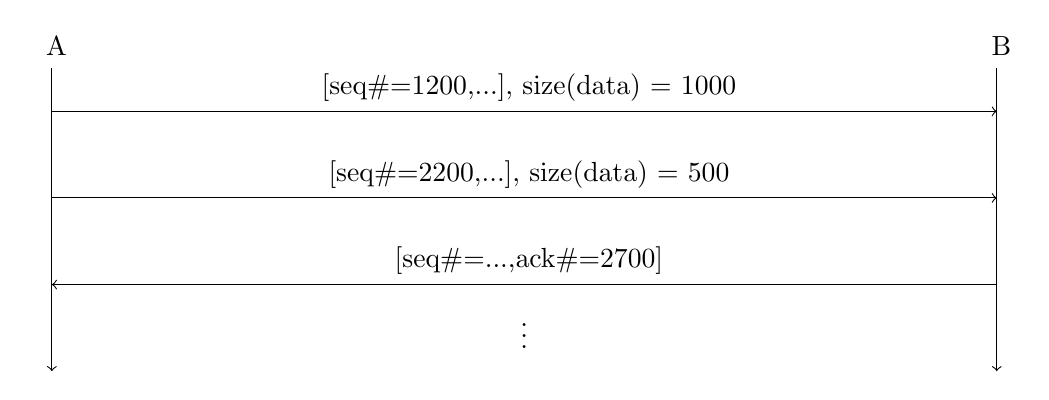
\begin{tikzpicture}[x=1.5cm, y=0.55cm]
                                \node at (4, -6) {$\vdots$};
                                \node at (0, 0.5) {~A~};
                                \node at (8, 0.5) {~B~};
                                \draw (0, 0) edge[->] (0, -7);
                                \draw (8, 0) edge[->] (8, -7);
                                \draw
                                (0, -1) edge[->, above] node{~[seq\#=1200,...], size(data) = 1000~} (8, -1)
                                (0, -3) edge[->, above] node{~[seq\#=2200,...], size(data) = 500~} (8, -3)
                                (8, -5) edge[->, above] node{~[seq\#=...,ack\#=2700]~} (0, -5);
                            \end{tikzpicture}
                        \end{center}
                        Note that because a TCP connection consists of a full-duplex link, there are two streams, hence two different sequence numbers (see the example below, of an "echo" application).
                        Acknowledgements are "piggybacked" on data segments.
                        \begin{center}
                            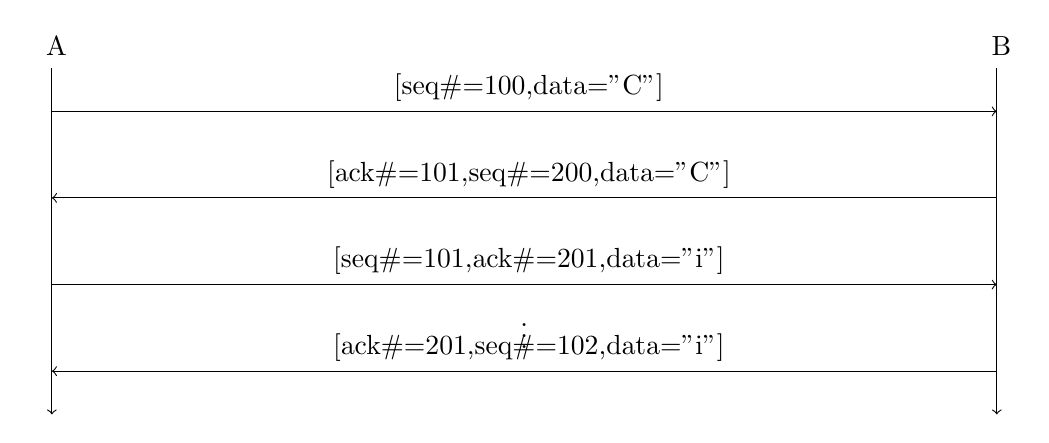
\begin{tikzpicture}[x=1.5cm, y=0.55cm]
                                \node at (4, -6) {$\vdots$};
                                \node at (0, 0.5) {~A~};
                                \node at (8, 0.5) {~B~};
                                \draw (0, 0) edge[->] (0, -8);
                                \draw (8, 0) edge[->] (8, -8);
                                \draw
                                (0, -1) edge[->, above] node{~[seq\#=100,data="C"]~} (8, -1)
                                (8, -3) edge[->, above] node{~[ack\#=101,seq\#=200,data="C"]~} (0, -3)
                                (0, -5) edge[->, above] node{~[seq\#=101,ack\#=201,data="i"]~} (8, -5)
                                (8, -7) edge[->, above] node{~[ack\#=201,seq\#=102,data="i"]~} (0, -7);
                            \end{tikzpicture}
                        \end{center}
                    \item receive window \hfill 16-bit (size of window on receiver end)
                    \item header length / offset \hfill 4-bit (size of TCP header in 32-bit words)
                    \item optional fields \hfill variable length (may be used to negotiate protocol parameters)
                    \item ~URG~ flag \hfill 1-bit (informs receiver some data is marked as urgent)
                    \item \violet{~ACK~ flag} \hfill 1-bit (value contained in the acknowledge number is a valid acknowledgement)
                        \medskip

                        See \textbf{acknowledgement number} above, and the \textbf{three-way handshake} section.
                    \item ~PSH~ flag \hfill 1-bit (solicit receiver to pass data to application immediately)
                    \item ~RST~ flag \hfill 1-bit (used during connection setup and shutdown)
                    \item \violet{~SYN~ flag} \hfill 1-bit (used during connection setup and shutdown)
                        \medskip

                        See the \textbf{three-way handshake} section below.
                    \item \violet{~FIN~ flag} \hfill 1-bit (used during connection shutdown)
                        \medskip

                        A client sends a TCP segment with ~FIN~ set, and the server responds with ~ACK~, and then the server sends a ~FIN~ TCP segment, client then responds with ~ACK~.
                        Closing a connection is simpler than initialising one.
                    \item \violet{checksum} \hfill 16-bit (used to detect transmission errors)
                \end{itemize}
            \subsubsection*{Three-Way Handshake}
                The three steps are as follows;
                \begin{enumerate}[1.]
                    \itemsep0em
                    \item \textbf{client} sends a TCP segment with ~SYN~ set, and an initial sequence number
                    \item \textbf{server} responds with another TCP segment with ~SYN~ set, as well as ~ACK~, the first unseen client sequence number, and the ISN for the server
                    \item \textbf{client} reserved with a TCP segment with ~ACK~ set, the first unseen server sequence number, and the client's new sequence number
                \end{enumerate}
                \begin{center}
                    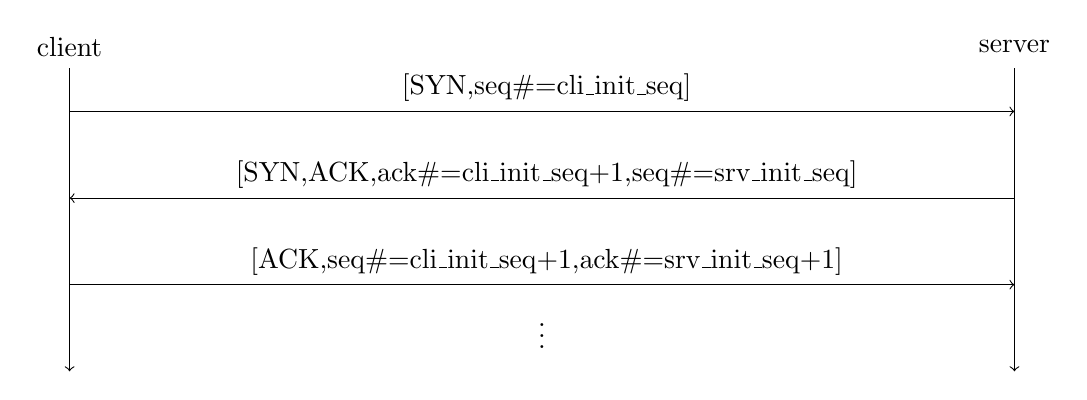
\begin{tikzpicture}[x=1.5cm, y=0.55cm]
                        \node at (4, -6) {$\vdots$};
                        \node at (0, 0.5) {client};
                        \node at (8, 0.5) {server};
                        \draw (0, 0) edge[->] (0, -7);
                        \draw (8, 0) edge[->] (8, -7);
                        \draw
                        (0, -1) edge[->, above] node{~[SYN,seq\#=cli\_init\_seq]~} (8, -1)
                        (8, -3) edge[->, above] node{~[SYN,ACK,ack\#=cli\_init\_seq+1,seq\#=srv\_init\_seq]~} (0, -3)
                        (0, -5) edge[->, above] node{~[ACK,seq\#=cli\_init\_seq+1,ack\#=srv\_init\_seq+1]~} (8, -5);
                    \end{tikzpicture}
                \end{center}
            \subsubsection*{User Datagram Protocol}
                UDP only provides the two most basic functions of a transport protocol, which are application identification (multiplexing and demultiplexing), and an integrity check via a CRC-type checksum.
                There is no flow control, no error control, nor any retransmissions.
                The datagrams cannot be larger than 65K, there is no segmentation, and the router will just drop it.
                The 65K consists of 20B IP header, 8B UDP header, 65507B of data, coming to a total of 65535 bytes.
                In practice, only 500 to 1000 bytes are used (the smaller the datagram, the more likely it will arrive intact).
                \medskip

                Instead of just using IP, it adds port numbers on top of it, allowing us to differentiate between applications.
                This is a connection-less protocol, therefore there is no need to connect (just send the data) but each datagram packet must carry the full address and port of the recipient.
                The UDP header consists of the following fields;
                \begin{itemize}
                    \itemsep0em
                    \item source and destination ports \hfill 16-bit each
                    \item length of data \hfill 16-bit
                    \item checksum \hfill 16-bit
                \end{itemize}
                Any application where we care more about speed, we can use UDP, since it is generally faster (due to the lack of connection establishment), and also has a smaller packet overhead.
            \subsubsection*{Berkeley Socket Interface}
                The \textbf{Berkeley} socket interface is as follows;
                \begin{itemize}
                    \itemsep0em
                    \item ~SOCKET~ \hfill create a new communication endpoint
                    \item ~BIND~ \hfill attach a local address to a socket
                        \subitem the client and server each bind a transport-level address and a name to the locally created socket
                    \item ~LISTEN~ \hfill announce willingness to accept ~N~ connections
                        \subitem server starts listening on this socket, thus telling the kernel it will wait for connections from clients
                    \item ~ACCEPT~ \hfill block until a remote client wishes to establish a connection
                        \subitem this blocks the current thread, thus it is a synchronous operation
                        \subitem from here the server can accept or select connections from clients
                    \item ~CONNECT~ \hfill attempt to establish a connection
                        \subitem a client connects to the socket, it needs to provide the full transport-level address to locate the socket
                    \item ~SEND~ \hfill send data over a connection
                    \item ~RECEIVE~ \hfill receive data over a connection
                        \subitem now the client and server communicate through these operations on their respective sockets
                    \item ~CLOSE~ \hfill release the connection
                        \subitem end the communication, must be closed otherwise connections may be continued, and may run out of ports
                \end{itemize}
                \begin{center}
                    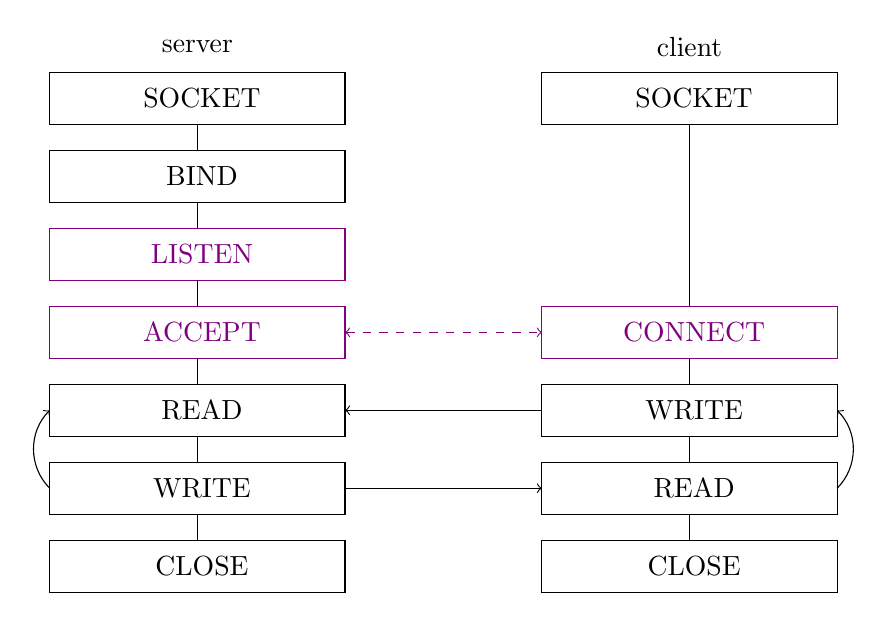
\begin{tikzpicture}[x=1.25cm, y=0.66cm]
                        \begin{scope}[shift={(0, 0)}]
                            \node at (1.5, 0.5) {server};
                            \node at (1.5, -0.5) {~SOCKET~};
                            \draw (0, 0) -- (3, 0) -- (3, -1) -- (0, -1) -- cycle;
                        \end{scope}
                        \begin{scope}[shift={(0, -1.5)}]
                            \node at (1.5, -0.5) {~BIND~};
                            \draw (0, 0) -- (3, 0) -- (3, -1) -- (0, -1) -- cycle;
                        \end{scope}
                        \begin{scope}[shift={(0, -3)}]
                            \node[violet] at (1.5, -0.5) {~LISTEN~};
                            \draw[violet] (0, 0) -- (3, 0) -- (3, -1) -- (0, -1) -- cycle;
                        \end{scope}
                        \begin{scope}[shift={(0, -4.5)}]
                            \node[violet] at (1.5, -0.5) {~ACCEPT~};
                            \draw[violet] (0, 0) -- (3, 0) -- (3, -1) -- (0, -1) -- cycle;
                        \end{scope}
                        \begin{scope}[shift={(0, -6)}]
                            \node at (1.5, -0.5) {~READ~};
                            \draw (0, 0) -- (3, 0) -- (3, -1) -- (0, -1) -- cycle;
                        \end{scope}
                        \begin{scope}[shift={(0, -7.5)}]
                            \node at (1.5, -0.5) {~WRITE~};
                            \draw (0, 0) -- (3, 0) -- (3, -1) -- (0, -1) -- cycle;
                        \end{scope}
                        \begin{scope}[shift={(0, -9)}]
                            \node at (1.5, -0.5) {~CLOSE~};
                            \draw (0, 0) -- (3, 0) -- (3, -1) -- (0, -1) -- cycle;
                        \end{scope}
                        \draw
                        (1.5, -1) -- (1.5, -1.5)
                        (1.5, -2.5) -- (1.5, -3)
                        (1.5, -4) -- (1.5, -4.5)
                        (1.5, -5.5) -- (1.5, -6)
                        (1.5, -7) -- (1.5, -7.5)
                        (1.5, -8.5) -- (1.5, -9)
                        (6.5, -1) -- (6.5, -4.5)
                        (6.5, -5.5) -- (6.5, -6)
                        (6.5, -7) -- (6.5, -7.5)
                        (6.5, -8.5) -- (6.5, -9)
                        (3, -5) edge[<->, dashed, violet] (5, -5)
                        (5, -6.5) edge[->] (3, -6.5)
                        (3, -8) edge[->] (5, -8)
                        (0, -8) edge[->, bend left=45] (0, -6.5)
                        (8, -8) edge[->, bend right=45] (8, -6.5);
                        \begin{scope}[shift={(5, 0)}]
                            \node at (1.5, 0.5) {client};
                            \node at (1.5, -0.5) {~SOCKET~};
                            \draw (0, 0) -- (3, 0) -- (3, -1) -- (0, -1) -- cycle;
                        \end{scope}
                        \begin{scope}[shift={(5, -4.5)}]
                            \node[violet] at (1.5, -0.5) {~CONNECT~};
                            \draw[violet] (0, 0) -- (3, 0) -- (3, -1) -- (0, -1) -- cycle;
                        \end{scope}
                        \begin{scope}[shift={(5, -6)}]
                            \node at (1.5, -0.5) {~WRITE~};
                            \draw (0, 0) -- (3, 0) -- (3, -1) -- (0, -1) -- cycle;
                        \end{scope}
                        \begin{scope}[shift={(5, -7.5)}]
                            \node at (1.5, -0.5) {~READ~};
                            \draw (0, 0) -- (3, 0) -- (3, -1) -- (0, -1) -- cycle;
                        \end{scope}
                        \begin{scope}[shift={(5, -9)}]
                            \node at (1.5, -0.5) {~CLOSE~};
                            \draw (0, 0) -- (3, 0) -- (3, -1) -- (0, -1) -- cycle;
                        \end{scope}
                    \end{tikzpicture}
                \end{center}
                Note that the part in \violet{violet} would not be present for UDP.
        \subsection*{30th January 2020 \hfill Week 4, Lecture 2}
            \subsubsection*{TCP vs UDP}
                The scenario is as follows; movie player app is being built that allows (paying) users to stream public domain movies.
                Since the users are paying, we should be using TCP, as it guarantees quality of service, whereas UDP does not.
                The difference in performance (TCP being slower than UDP) can be circumvented by pre-buffering (sending some data in advance for the client to store locally).
                This however doesn't work for live events - we can either switch to UDP, or introduce a delay between the feed and the live event.
            \subsubsection*{QUIC}
                QUIC (Quick UDP Internet Connections) is a new layer 4 protocol, implemented by a Google engineer in 2012.
                Originally, it was designed for general purpose, but now it is being used for HTTP (layer 5).
                This is still a draft, but is actively being used by some web servers.
            \subsubsection*{Finite-State Machines}
                A finite-state machine (FSM) is a mathematical abstraction, where states are represented as nodes, and transitions are directed edges between states, labelled with events.
                They are also known as finite-state automaton (FSA), deterministic finite-state automaton (DFA), and non-deterministic finite-state automaton (NFA) - multiple edges with the same label from one node.
                This can be used to specify protocols, where the states represent the state of a protocol, and transitions are characterised by an event / action label (event typically consists of an input message or timeout, whereas an action typically consists of an output message).
                $$\frac{\text{input / timeout (event)}}{\text{output (action)}}$$
                Examples of this are in the slides, for the TCP state machines for both the client and server.
            \subsubsection*{Reliable Data Transfer}
                TCP adds a reliable channel on top of an unreliable channel (IP) which is "best effort" delivery.
                The service provided by the transport layer sits on top of the service provided by the network layer.
                \begin{center}
                    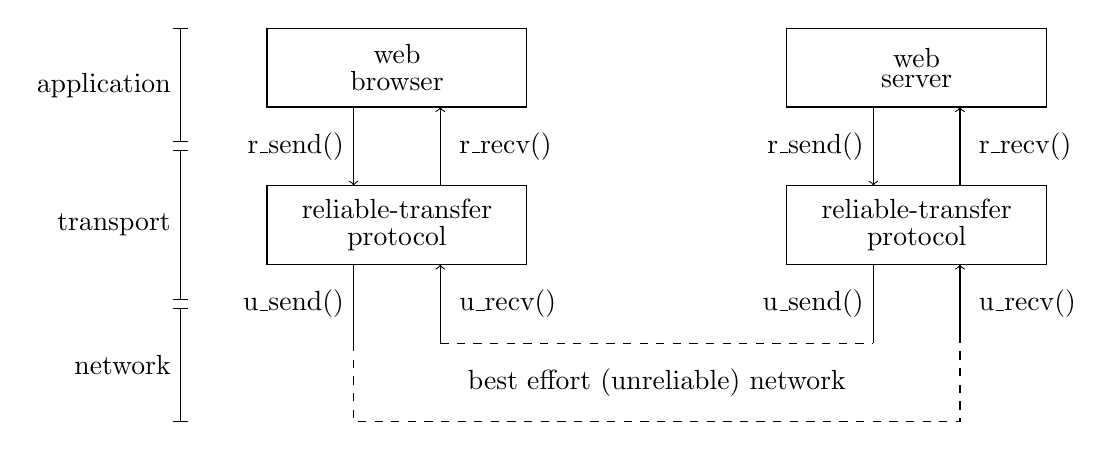
\begin{tikzpicture}[x=1.1cm, y=0.5cm]
                        \node at (1.5, -1) {\shortstack{web\\browser}};
                        \node at (7.5, -1) {\shortstack{web\\server}};
                        \begin{scope}[shift={(0, 0)}]
                            \begin{scope}[shift={(0, 0)}]
                                \draw (0, 0) -- (3, 0) -- (3, -2) -- (0, -2) -- cycle;
                            \end{scope}
                            \begin{scope}[shift={(0, -4)}]
                                \node at (1.5, -1) {\shortstack{reliable-transfer\\protocol}};
                                \draw (0, 0) -- (3, 0) -- (3, -2) -- (0, -2) -- cycle;
                            \end{scope}
                            \draw
                            (1, -2) edge[->, left] node{~r\_send()~} (1, -4)
                            (1, -6) edge[left] node{~u\_send()~} (1, -8)
                            (2, -4) edge[->, right] node{~r\_recv()~} (2, -2)
                            (2, -8) edge[->, right] node{~u\_recv()~} (2, -6);
                        \end{scope}
                        \node at (4.5, -9) {best effort (unreliable) network};
                        \draw[dashed]
                        (2, -8) -- (7, -8)
                        (1, -8) -- (1, -10) -- (8, -10) -- (8, -8);
                        \draw
                        (-1, 0) edge[|-|, left] node{application} (-1, -2.9)
                        (-1, -3.1) edge[|-|, left] node{transport} (-1, -6.9)
                        (-1, -7.1) edge[|-|, left] node{network} (-1, -10);
                        \begin{scope}[shift={(6, 0)}]
                            \begin{scope}[shift={(0, 0)}]
                                \draw (0, 0) -- (3, 0) -- (3, -2) -- (0, -2) -- cycle;
                            \end{scope}
                            \begin{scope}[shift={(0, -4)}]
                                \node at (1.5, -1) {\shortstack{reliable-transfer\\protocol}};
                                \draw (0, 0) -- (3, 0) -- (3, -2) -- (0, -2) -- cycle;
                            \end{scope}
                            \draw
                            (1, -2) edge[->, left] node{~r\_send()~} (1, -4)
                            (1, -6) edge[left] node{~u\_send()~} (1, -8)
                            (2, -4) edge[->, right] node{~r\_recv()~} (2, -2)
                            (2, -8) edge[->, right] node{~u\_recv()~} (2, -6);
                        \end{scope}
                    \end{tikzpicture}
                \end{center}
                Another issue is transmitting data through a noisy channel.
                There is a chance no packets will be lost, but a a bit may be modified during the transmission (flipped).
                The stages of dealing with this are as follows;
                \begin{itemize}
                    \itemsep0em
                    \item \textbf{error detection} \hfill receiver must know when a received packet is corrupted
                        \medskip

                        Some strategies for detecting errors are as follows;
                        \begin{itemize}
                            \itemsep0em
                            \item sending redundant information
                                \subitem sending information twice, report an error if two different messages received - inefficient
                            \item error-detection codes
                                \subitem parity bit, adding a single bit at the end that is the XOR of all other bits in the message, if the recomputed XOR (by receiver) is different, then an error occurred
                        \end{itemize}
                    \item \textbf{receiver feedback} \hfill receiver must be able to alert sender that a corrupted packet was received
                        \medskip

                        ~ACK~s and ~NACK~s are also protected with an error-detection code, with corrupted ~ACK~s being treated as ~NACK~s.
                        This may possibly generate duplicate segments, however sequence numbers allow the receiver to ignore these data segments.
                    \item \textbf{retransmission} \hfill the sender must retransmit corrupted packets
                \end{itemize}
                Note that in the diagram below, ~[data]*~ indicates a packet containing ~data~ and an error-detection code, and $A$ represents the acknowledgement state.
                \begin{center}
                    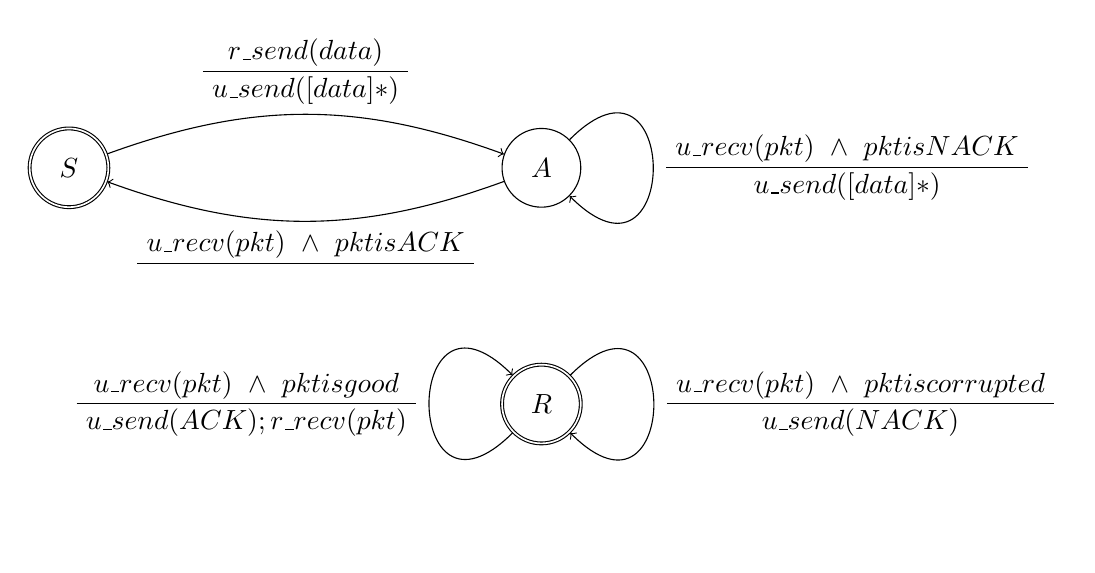
\begin{tikzpicture}
                        \node[state, minimum size=1cm, accepting] (s) at (0, 0) {$S$};
                        \node[state, minimum size=1cm] (a) at (6, 0) {$A$};
                        \draw
                        (s) edge[->, bend left=20, above] node{$\dfrac{~r\_send(data)~}{~u\_send([data]*)~}$} (a)
                        (a) edge[->, bend left=20, below] node{$\dfrac{~u\_recv(pkt)~ \land ~pkt is ACK~}{}$} (s)
                        (a) edge[->, loop, out=45, in=-45, distance=2cm, right] node{$\dfrac{~u\_recv(pkt)~ \land ~pkt is NACK~}{~u\_send([data]*)~}$} (a);
                        \node[state, minimum size=1cm, accepting] (r) at (6, -3) {$R$};
                        \draw
                        (r) edge[->, loop, out=45, in=-45, distance=2cm, right] node{$\dfrac{~u\_recv(pkt)~ \land ~pkt is corrupted~}{~u\_send(NACK)~}$} (r)
                        (r) edge[->, loop, out=225, in=135, distance=2cm, left] node{$\dfrac{~u\_recv(pkt)~ \land ~pkt is good~}{~u\_send(ACK); r\_recv(pkt)~}$} (r);
                    \end{tikzpicture}
                \end{center}
                This is a synchronous (or stop-and-wait) for each segment, as the sender must receive a positive acknowledgement before it can take more data from the application layer.
                However, this can have issues when the ~ACK/NACK~ packets have issues.
                A way around this is for the sender to add a sequence number to each packet, thus allowing the receiver to determine whether a packet is a retransmission.
                If the sender does not hear an acknowledgement, due to some failure, it assumes a ~NACK~, and retransmits.
                However, if the receiver did actually send an acknowledgement, it would ignore the packet, since it knows it is a retransmission.
                It then resends the ~ACK~, and doesn't process the retransmitted.
                \medskip

                Since this is a stop-and-wait protocol for each segment, only one bit is needed for the sequence number - as all we need to do is distinguish between the next segment and the retransmission of the current segment.
                \medskip

                However, now that we have sequence numbers, we don't need both ~ACK~ and ~NACK~, since we can convey the same semantics by sending an ~ACK~ for the last good packet it received.
                \begin{center}
                    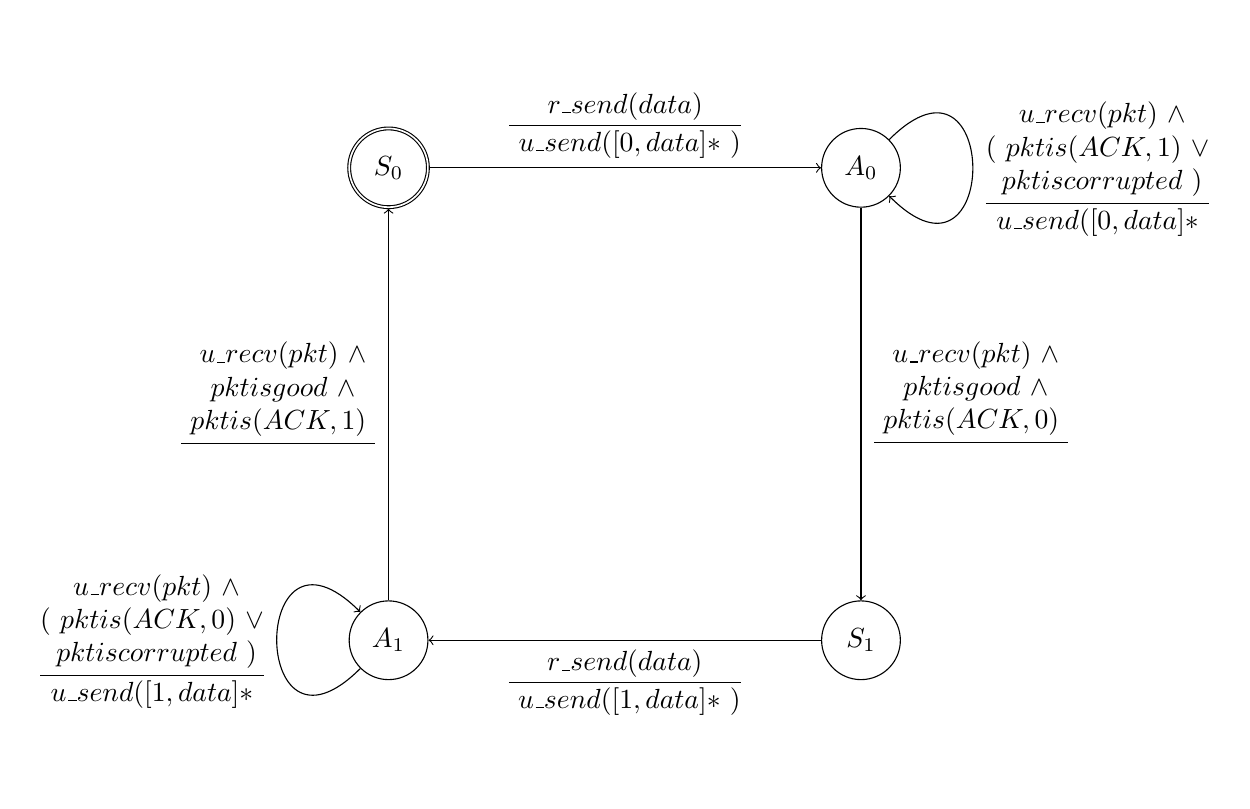
\begin{tikzpicture}
                        \node[state, minimum size=1cm, accepting] (s0) at (0, 0) {$S_0$};
                        \node[state, minimum size=1cm] (a0) at (6, 0) {$A_0$};
                        \node[state, minimum size=1cm] (s1) at (6, -6) {$S_1$};
                        \node[state, minimum size=1cm] (a1) at (0, -6) {$A_1$};
                        \draw
                        (s0) edge[->, above] node{$\dfrac{~r\_send(data)~}{~u\_send([0, data]*~)}$} (a0)
                        (a0) edge[->, right] node{$\dfrac{\begin{matrix}
                            ~u\_recv(pkt) ~ \land \\
                            ~pkt is good ~ \land \\
                            ~pkt is (ACK, 0)~
                        \end{matrix}}{}$} (s1)
                        (s1) edge[->, below] node{$\dfrac{~r\_send(data)~}{~u\_send([1, data]*~)}$} (a1)
                        (a1) edge[->, left] node{$\dfrac{\begin{matrix}
                            ~u\_recv(pkt) ~ \land \\
                            ~pkt is good ~ \land \\
                            ~pkt is (ACK, 1)~
                        \end{matrix}}{}$} (s0)
                        (a0) edge[->, loop, in=-45, out=45, distance=2cm, right] node{$\dfrac{\begin{matrix}
                            ~u\_recv(pkt) ~ \land \\
                            (~pkt is (ACK, 1) ~ \lor \\
                            ~pkt is corrupted~)
                        \end{matrix}}{~u\_send([0, data]*~}$} (a0)
                        (a1) edge[->, loop, in=135, out=225, distance=2cm, left] node{$\dfrac{\begin{matrix}
                            ~u\_recv(pkt) ~ \land \\
                            (~pkt is (ACK, 0) ~ \lor \\
                            ~pkt is corrupted~)
                        \end{matrix}}{~u\_send([1, data]*~}$} (a1);
                    \end{tikzpicture}
                \end{center}
                \begin{center}
                    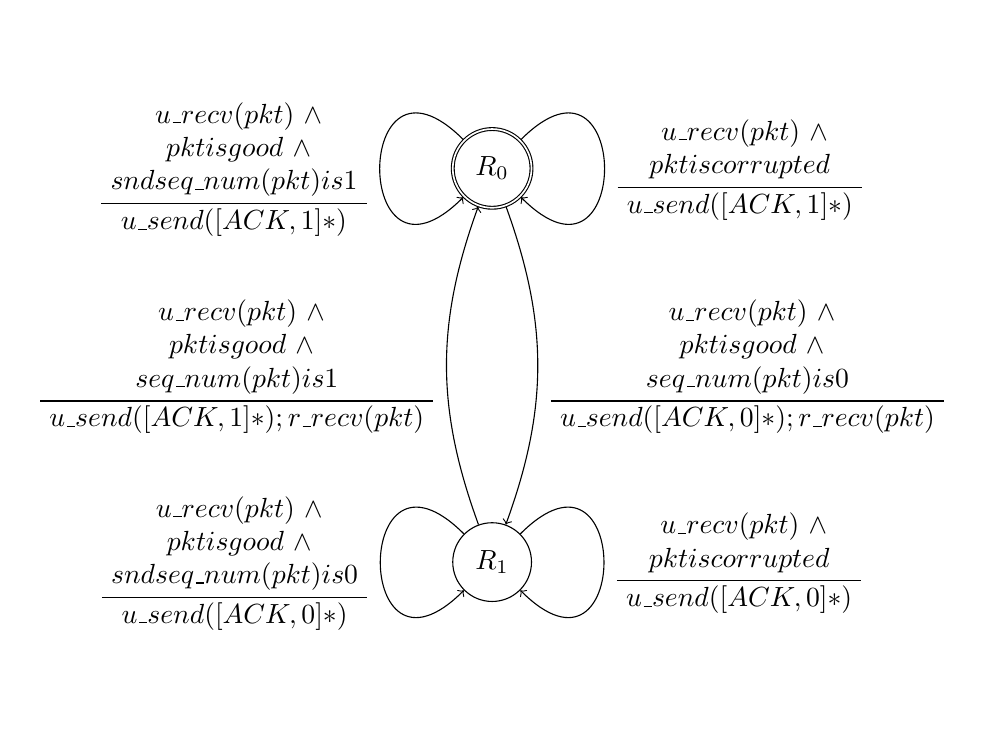
\begin{tikzpicture}
                        \node[state, minimum size=1cm, accepting] (r0) at (0, 0) {$R_0$};
                        \node[state, minimum size=1cm] (r1) at (0, -5) {$R_1$};

                        \draw
                        (r0) edge[->, bend left=20, right] node{$\dfrac{\begin{matrix}
                            ~u\_recv(pkt) ~ \land \\
                            ~pkt is good ~ \land \\
                            ~seq\_num(pkt) is 0~
                        \end{matrix}}{~u\_send([ACK, 0]*); r\_recv(pkt)~}$} (r1)
                        (r1) edge[->, bend left=20, left] node{$\dfrac{\begin{matrix}
                            ~u\_recv(pkt) ~ \land \\
                            ~pkt is good ~ \land \\
                            ~seq\_num(pkt) is 1~
                        \end{matrix}}{~u\_send([ACK, 1]*); r\_recv(pkt)~}$} (r0)
                        (r0) edge[->, loop, out=45, in=-45, distance=2cm, right] node{$\dfrac{\begin{matrix}
                            ~u\_recv(pkt) ~ \land \\
                            ~pkt is corrupted~
                        \end{matrix}}{~u\_send([ACK, 1]*)~}$} (r0)
                        (r1) edge[->, loop, out=45, in=-45, distance=2cm, right] node{$\dfrac{\begin{matrix}
                            ~u\_recv(pkt) ~ \land \\
                            ~pkt is corrupted~
                        \end{matrix}}{~u\_send([ACK, 0]*)~}$} (r1)
                        (r0) edge[->, loop, out=135, in=225, distance=2cm, left] node{$\dfrac{\begin{matrix}
                            ~u\_recv(pkt) ~ \land \\
                            ~pkt is good ~ \land \\
                            ~snd seq\_num(pkt) is 1~
                        \end{matrix}}{~u\_send([ACK, 1]*)~}$} (r0)
                        (r1) edge[->, loop, out=135, in=225, distance=2cm, left] node{$\dfrac{\begin{matrix}
                            ~u\_recv(pkt) ~ \land \\
                            ~pkt is good ~ \land \\
                            ~snd seq\_num(pkt) is 0~
                        \end{matrix}}{~u\_send([ACK, 0]*)~}$} (r1);
                    \end{tikzpicture}
                \end{center}
            \subsubsection*{Acknowledgement Generation}
                The following are cases of segment arrival, and how the protocol handles them;
                \begin{itemize}
                    \itemsep0em
                    \item arrival of in-order segment with expected sequence number (all data up to expected sequence number already acknowledged)
                        \subitem delayed ~ACK~, wait up to 500ms for another in-order segment, if it doesn't arrive, send ~ACK~ for just this segment
                    \item arrival of in-order segment with expected sequence number (one other in-order segment awaiting ~ACK~, from above case)
                        \subitem immediately send cumulative ~ACK~ for both segments
                    \item arrival of out of order segment with higher-than-expected sequence number (gap detected)
                        \subitem immediately send duplicate ~ACK~ - the sender will know to fill in the gap, as it would've already seen this acknowledgement
                    \item arrival of segment that fills a gap in the received data
                        \subitem immediately send ~ACK~ if segment starts at lower end of gap
                \end{itemize}
                Additionally, it's important to note that lost packets can easily be treated as corrupted packets.
                Since I don't really want to draw the FSM again, add a ~start\_timer()~ after every ~u\_send(...)~, and an additional transition loop to $A_0$ and $A_1$, which sends the same data, but the input is ~timeout~.
                \medskip

                There's also a small section after this on the alternating bit protocol, which isn't used in practice.
        \subsection*{30th January 2020 \hfill Week 4, Lecture 3}
            \subsubsection*{Congestion Detection}
                If the queue of one or more routers between the sender and receiver overflow, we call it \textbf{congestion} - this has the visible effect of segments being dropped.
                The server can assume the network experiences congestion when it detects a segment loss; either on a timeout, hence no ~ACK~, or multiple acknowledgements, which is equivalent to ~NACK~.
                \medskip

                TCP we've described so far is referred to as TCP Reno.
                Another popular implementation is TCP Vegas, which aims to detect congestion before losses occur.
                It does this by predicting imminent packet loss via observing the RTT - the longer it is, the greater the congestion in the routers.
                However, flows with small RTTs are advantaged, compared to the ones with large RTTs, as their window can grow faster.
                TCP CUBIC circumvents this by making the window increase as a function of time rather than RTT.
            \subsubsection*{Congestion Window and Congestion Control}
                The congestion window, $W$, is maintained by the sender, and limits the amount of bytes that the sender pushes into the network before it blocks to wait for acknowledgements.
                \begin{center}
                    $\text{LastByteSent} - \text{LastByteAcked} \leq W = \min(\text{CongestionWindow}, \text{ReceiverWindow})$
                \end{center}
                This gives a resulting maximum output of roughly
                $$\lambda = \frac{W}{\text{RTT}}$$
                The phases are as follows;
                \begin{itemize}
                    \itemsep0em
                    \item \textbf{slow start}
                        \medskip

                        The initial value of $W$ is the maximum segment size (MSS), which is quite low for modern (high-speed) networks.
                        To result in a good throughput, TCP increases the sending rate exponentially for its first phase.
                        It increases $W$ by 1 MSS on every (positive) segment acknowledgement (doubles each time - the first ~ACK~ increases it by 1 MSS, the second ~ACK~ will be after sending 2 segments, hence it increases by a further s2 MSS, and so on), until it reaches some slow start threshold (ssthresh), or until congestion occurs.
                        If $W$ is greater than (ssthresh), then use congestion avoidance (if they are equal, either could be used).
                    \item \textbf{congestion avoidance}
                        \medskip

                        TCP then increases $W$ linearly in this phase.
                        $$W = W + \underbrace{\text{MSS} \cdot \frac{\text{MSS}}{W}}_\text{increment}$$
                        This happens until congestion is detected.
                    \item \textbf{Additive-Increase / Multiplicative-Decrease (AIMD)}
                        \begin{itemize}
                            \itemsep0em
                            \item at every good acknowledgement, increase $W$ in accordance with congestion avoidance ($\frac{\text{MSS}^2}{W}$)
                            \item at every packet loss event, TCP halves the congestion window
                                \medskip

                                There are two possibilities for packet loss.
                                TCP provides reliable data transfer by using a timer to detect lost segments.
                                If there is a timeout, without an ~ACK~, it means that there is likely a lost packet, hence a retransmission is required.
                                This timeout interval, $T$, must be larger than the RTT to avoid unnecessary retransmissions, however it shouldn't be too far from RTT, as we want to detect and retransmit lost segments as quickly as possible.
                                TCP sets its timeouts as follows, where (1) is the estimated RTT, and (2) is the variability estimate;
                                $$T = \underbrace{\overline{\text{RTT}}}_{(1)} + 4 \cdot \underbrace{\overline{\text{DevRTT}}}_{(2)}$$
                                The timeout is controlled by continuously estimating the current RTT.
                                \medskip

                                The agreement is that 3 duplicate ~ACK~s (hence 4 identical ~ACK~s overall), are interpreted as a ~NACK~ in \textbf{fast retransmit}.
                                While both timeouts and ~NACK~s signal a loss, they say different things about the status of the network, hence TCP should react differently.
                                A timeout indicates congestion, whereas the duplicate ~ACK~s suggests the network is able to still able to deliver segments along that path.
                                \medskip

                                In the formulae below, assume the current window size is $W = \overline{W}$;
                                \begin{itemize}
                                    \itemsep0em
                                    \item timeout
                                        \medskip

                                        In the event of a timeout, set $W = \text{MSS}$, and run slow start until $W$ reaches $\frac{\overline{W}}{2}$ (which is the new ssthresh), and then proceed with congestion avoidance.
                                    \item ~NACK~
                                        \medskip

                                        Similarly set ssthresh to $\frac{\overline{W}}{2}$, but set $W = \frac{\overline{W}}{2}$.
                                        We then continue to run congestion avoidance, which increases $W$ linearly - \textbf{fast recovery}.
                                \end{itemize}
                        \end{itemize}
                \end{itemize}
            \subsubsection*{Selective Repeat}
                The sender only transmits packets it suspects were lost or corrupted.
                However, if we were to use a TCP flavour that uses this, we'd need powerful routers in the path, as it requires storage and processing.
                \begin{itemize}
                    \itemsep0em
                    \item sender maintains a vector of acknowledgement flags
                    \item receiver maintains a vector of acknowledged flags
                        \subitem maintains a buffer of out-of-order packets
                    \item sender maintains a timer for each pending packet
                    \item sender resends a packet when its timer experiences
                    \item sender slides the window when the lowest pending sequence number is acknowledged
                \end{itemize}
                \begin{center}
                    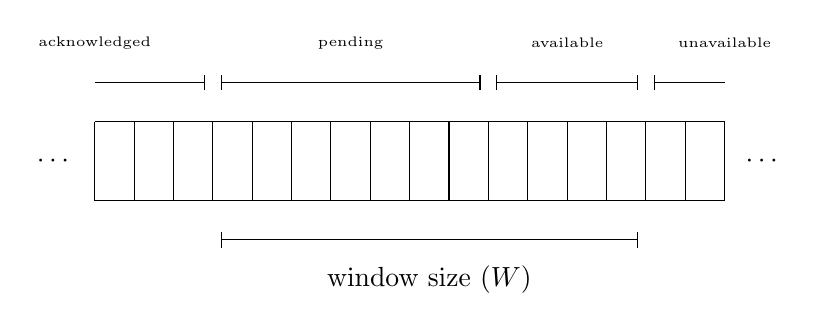
\begin{tikzpicture}
                        \draw
                        (0, 0) -- (8, 0)
                        (0, -1) -- (8, -1);
                        \foreach \x in {0,...,16} {
                            \draw (0 + 0.5*\x, -1) -- (0 + 0.5*\x, 0);
                        }
                        \draw
                        (0, 0.5) edge[-|] (1.4, 0.5)
                        (1.6, 0.5) edge[|-|] (4.9, 0.5)
                        (5.1, 0.5) edge[|-|] (6.9, 0.5)
                        (7.1, 0.5) edge[|-] (8, 0.5)
                        (1.6, -1.5) edge[|-|] (6.9, -1.5);

                        \node at (-0.5, -0.5) {$\cdots$};
                        \node at (8.5, -0.5) {$\cdots$};
                        \node at (0, 1) {\tiny{acknowledged}};
                        \node at (3.25, 1) {\tiny{pending}};
                        \node at (6, 1) {\tiny{available}};
                        \node at (8, 1) {\tiny{unavailable}};
                        \node at (4.25, -2) {window size ($W$)};
                    \end{tikzpicture}
                \end{center}
            \subsubsection*{Flow Control vs Congestion Control}
                The former aims to not overflow the receiver, whereas the latter aims not to overflow the network.
                An example of flow control is as follows;
                \begin{center}
                    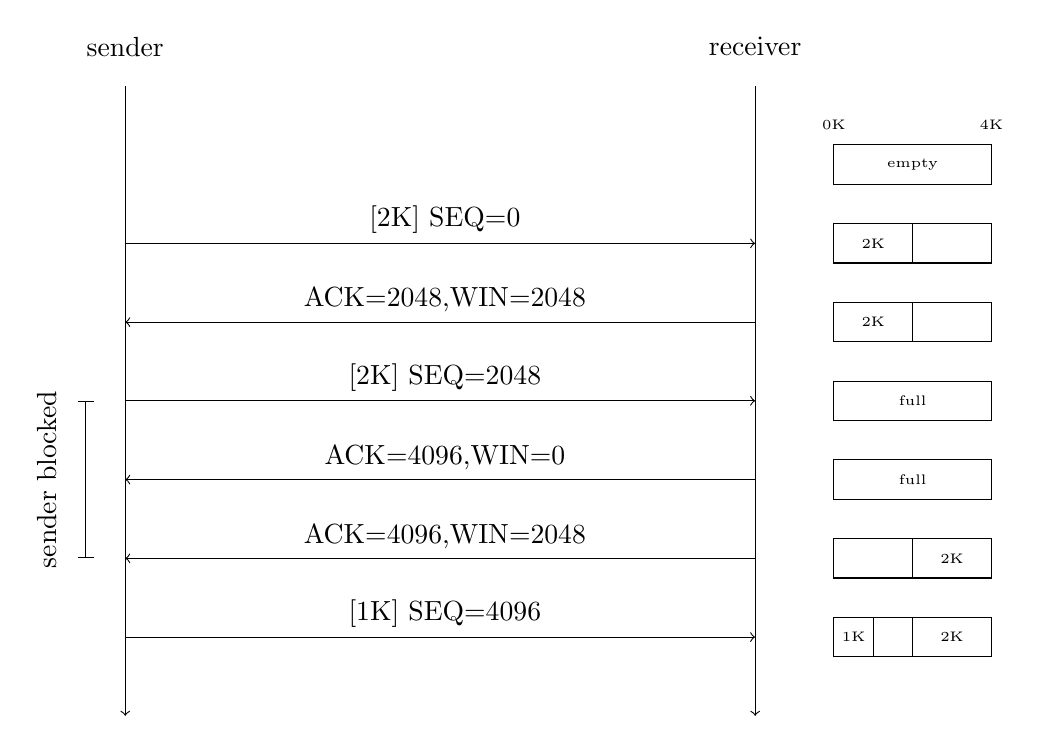
\begin{tikzpicture}
                        \node at (0, 1.5) {sender};
                        \node at (8, 1.5) {receiver};
                        \foreach \y in {0,...,6} {
                            \draw (9, 0.25 - \y) -- (11, 0.25 - \y) -- (11, -0.25 - \y) -- (9, -0.25 - \y) -- cycle;
                        }
                        \node at (9, 0.5) {\tiny{0K}};
                        \node at (11, 0.5) {\tiny{4K}};
                        \node at (10, 0) {\tiny{empty}};
                        \node at (9.5, -1) {\tiny{2K}};
                        \node at (9.5, -2) {\tiny{2K}};
                        \node at (10, -3) {\tiny{full}};
                        \node at (10, -4) {\tiny{full}};
                        \node at (10.5, -5) {\tiny{2K}};
                        \node at (9.25, -6) {\tiny{1K}};
                        \node at (10.5, -6) {\tiny{2K}};
                        \draw
                        (10, -0.75) -- (10, -1.25)
                        (10, -1.75) -- (10, -2.25)
                        (10, -4.75) -- (10, -5.25)
                        (9.5, -5.75) -- (9.5, -6.25)
                        (10, -5.75) -- (10, -6.25);
                        \draw
                        (0, 1) edge[->] (0, -7)
                        (8, 1) edge[->] (8, -7);
                        \draw
                        (0, -1) edge[->, above] node{~[2K] SEQ=0~} (8, -1)
                        (8, -2) edge[->, above] node{~ACK=2048,WIN=2048~} (0, -2)
                        (0, -3) edge[->, above] node{~[2K] SEQ=2048~} (8, -3)
                        (8, -4) edge[->, above] node{~ACK=4096,WIN=0~} (0, -4)
                        (8, -5) edge[->, above] node{~ACK=4096,WIN=2048~} (0, -5)
                        (0, -6) edge[->, above] node{~[1K] SEQ=4096~} (8, -6);
                        \node[rotate=90] at (-1, -4) {sender blocked};
                        \draw (-0.5, -3) edge[|-|] (-0.5, -5);
                    \end{tikzpicture}
                \end{center}
                The receiver sends the maximum number of bytes that may be sent (ReceiverWindow) along with the acknowledgement - a size of 0 is legal, and it means no more messages can be sent, except a 1-byte segment to ping receivers.
            \subsubsection*{Wireless TCP}
                TCP assumes that IP is running across wires.
                Therefore, when packets are lost, it assumes that this is due to congestion and slows down, whereas in wireless environments, packets are usually lost to channel reliability issues (where TCP should actually try harder).
                \medskip

                One solution it to split TCP connections to distinguish between wired and wireless IP.
                Another solution would be to allow the base station to do some retransmission, without informing the source (if it still fails, the source is then informed).
            \subsubsection*{Network Usage}
                We can quantify network usage with the utilisation factor;
                $$\frac{\text{how much we actually used the network}}{\text{how much we could have used it}}$$
                For example, if we were to rent a 24Mbps line, and download at 2MBps, we are at around 67\% utilisation (note the conversion from bits to bytes).
                This may be due to congestion control and / or flow control, as it may not be possible for all nodes in the route to support the amount of traffic you wish to send.
                \medskip

                If we have all the data, we can use the following formula for utilisation;
                $$U = \frac{\frac{L}{R}}{\text{RTT} + \frac{L}{R}}$$
                For example, if we have a RTT of 30ms, a channel with transmission rate $R = 1\text{Gbps}$, and a packet size $L = 1000 \text{bits}$, we have a utilisation of $U \approx 0.027\%$.
        \subsection*{4th February 2020 \hfill Week 5, Lecture 1}
            \subsubsection*{H/P/V/A/C}
                \begin{itemize}
                    \itemsep0em
                    \item \textbf{hackers}
                        \medskip

                        Originally meant highly competent computer engineers who explore different ways of using / combining things.
                        Can be divided into the following;
                        \begin{itemize}
                            \itemsep0em
                            \item white hat \hfill a researcher who informs the company of problems before they go public
                            \item grey hat \hfill an analyst who does not inform anyone unless they get paid
                            \item black hat \hfill a malicious individual who abuses the findings to cause harm
                        \end{itemize}
                    \item \textbf{phreakers}
                        \medskip

                        Phone hackers - not as prevalent anymore, due to the telephone network being almost fully digital.
                        Playing the right frequencies allowed for access to administrative interface for a phone network.
                    \item \textbf{virii (creators)}
                        \medskip

                        Create viruses, for curiosity or money.
                        Popular viruses include ransomware, spyware, and Trojans (remotely controlled botnet, and profit from renting).
                        A rootkit is injected into the root account, running as the superuser, thus having more control.
                    \item \textbf{anarchists} \hfill "hacktivists"
                    \item \textbf{crackers}
                        \medskip

                        Originally meant wannabe hackers (script kiddies), who use the tools of others to infiltrate systems.
                \end{itemize}
            \subsubsection*{Methods and Tools}
                Some commonly used methods are as follows;
                \begin{itemize}
                    \itemsep0em
                    \item \textbf{credential reuse / stuffing} \hfill leaked ~email:password~ combinations tested on other services
                    \item \textbf{network monitor / packet sniffing} \hfill reading messages not intended for your NIC
                    \item \textbf{code / SQL injection} \hfill running your own code in someone else's system
                    \item \textbf{session / cookie hijacking} \hfill use another session without credentials
                    \item \textbf{wardriving} \hfill searching and using unsecured WiFi spots
                    \item \textbf{dumpster diving / trashing} \hfill physically checking trash for information
                    \item \textbf{clickjacking} \hfill forcing users to click on hidden links
                    \item \textbf{bat and switch} \hfill legitimate-looking ads leading to malicious destinations
                    \item \textbf{spoofing} \hfill IP (layer 3), MAC (layer 2), DNS poisoning
                \end{itemize}
                Some commonly used tools are as follows;
                \begin{itemize}
                    \itemsep0em
                    \item \textbf{rootkit} \hfill runs as an administrator (can reinstall itself)
                    \item \textbf{keyloggers} \hfill allows attackers to record all keypresses
                    \item \textbf{trojans} \hfill allows attackers to remote control an entire system (similar to \textit{TeamViewer} or VNC)
                    \item \textbf{TAILS} \hfill The Amnesic Incognito Live System - forgets on reboot
                    \item \textbf{Kali Linux} \hfill large collection of security and pentesting tools
                    \item \textbf{Metasploit} \hfill identifies systems and their vulnerabilities (similar to nmap)
                \end{itemize}
            \subsubsection*{Laws and Standards}
                Basically just a long list of laws (and their years), and organisations.
                \begin{itemize}
                    \itemsep0em
                    \item Computer Misuse Act (1990) \hfill most intrusions fall under this
                    \item Copyright, Designs, and Patents Act (1988) \hfill piracy
                    \item Criminal Justice Act (2003)
                    \item Data Protection Act (2018)
                    \item Defamation Act (2013) \hfill cyber-bullying
                    \item Disability Discrimination Act (2005)
                    \item Freedom of Information Act (2000) \hfill can be used against companies
                    \item Obscene Publications Act (1964)
                    \item Protection of Children Act (1978) \hfill 1999 version still being amended
                    \item Regulation of Investigatory Powers Act (2000)
                \end{itemize}
                Note that an intruder is trialled in both the country they reside in, as well as the laws of the country where the involved hosts are physically located.
                \begin{itemize}
                    \itemsep0em
                    \item IANA (Internet Assigned Numbers Authority) \hfill sets these standards, and assigns port numbers
                    \item ICANN (Internet Corporation for Assigned Numbers and Names) \hfill names for corporations
                    \item IETF (Internet Engineering Task Force) \hfill attempt to set standards straight
                    \item ISOC (Internet Society) \hfill push governments to update laws
                    \item EFF (Electronic Frontier Foundation) \hfill push rights (free speech and equality) online
                    \item W3C (World Wide Web Consortium)
                    \item ISO (International Organisation for Standardisation)
                \end{itemize}
        \subsection*{6th February 2020 \hfill Week 5, Lecture 2}
            \subsubsection*{Examples}
                Some examples include Heartbleed, KRACK, and some other legal / ethical grey areas.
                GDPR forces companies to inform their users of hacks within 72 hours.
            \subsubsection*{Network Security Issues}
                We want control access over a channel between a user and a resource.
                We need a way to ensure only specific users can access a resource (access control), as well as a way to authenticate the user (and resource).
                Additionally, confidentiality also has to be ensured to limit access to information owned by users, as well as integrity (actions of a user should not be able to affect the overall integrity of a resource).
                Users also cannot deny communication took place (non-repudiation) - blockchain is an example.
                To achieve this we need;
                \begin{itemize}
                    \itemsep0em
                    \item access control
                    \item security policy
                    \item secure channel (users and data are authenticated, information exchanged is confidential)
                    \item monitoring / logging / auditing
                \end{itemize}
            \subsubsection*{Access Control}
                \begin{center}
                    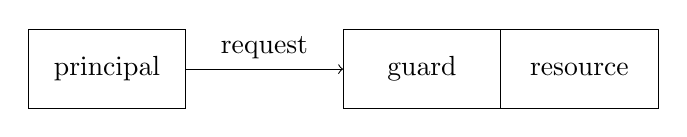
\begin{tikzpicture}
                        \draw
                        (0, 0) -- (2, 0) -- (2, -1) -- (0, -1) -- cycle
                        (4, 0) -- (8, 0) -- (8, -1) -- (4, -1) -- cycle
                        (6, 0) -- (6, -1)
                        (2, -0.5) edge[->, above] node {request} (4, -0.5);
                        \node at (1, -0.5) {principal};
                        \node at (5, -0.5) {guard};
                        \node at (7, -0.5) {resource};
                    \end{tikzpicture}
                \end{center}
                Assuming a secure channel, the guard controls which principals can access the resource, where principals are allowed to be located (access within networks), and what requests (actions) principals are allowed to make.
                \medskip

                This is done via the use of a \textbf{firewall}, which controls access to the network by providing a security gateway between the internal and external networks.
                \begin{itemize}
                    \itemsep0em
                    \item \textbf{application-level gateway} \hfill runs on the host, and only protects that host (such as iptables)
                        \medskip

                        This is in a logical connection, allowing it to monitor traffic.
                        This means that it can block / filter / report based on application level message content (as well as scan for data leaks, viruses, etc).
                        Data can also be rewritten, therefore we do not want this to be compromised.
                        If the data is encrypted, it may ask for the ability to read it, thus decrypting it, and then re-encrypting it for the client.
                    \item \textbf{proxy server} \hfill runs on network, and can protect entire LAN
                        \medskip

                        Proxies can filter incoming / outgoing traffic in different modes;
                        \begin{itemize}
                            \itemsep0em
                            \item \textbf{normal} \hfill client is aware (and needs to be set up)
                            \item \textbf{transparent} \hfill client is unaware (local router takes care of everything)
                            \item \textbf{reverse} \hfill runs on receiving side, impersonates servers (CDN load balancing)
                        \end{itemize}
                        SOCKS proxies can be used for any protocol, whereas HTTP is for web.
                    \item \textbf{circuit-level gateway} \hfill takes over host's communication as a non-caching proxy (such as Tor)
                    \item \textbf{stateless packet filtering} \hfill checks source / destination IP addresses and ports
                    \item \textbf{stateful packet filtering} \hfill checks contents of current and previous packets
                        \medskip

                        It can also perform user authentication.
                        Connections can be dropped based on destination, incorrect packets, time, or volume.
                        This is done with inspection to the layer 4 ports, layer 3 IP addresses, and the layer 2 MAC addresses.
                \end{itemize}
                The \textbf{Bastion} host is the host that all public connections arrive to.
                It should expect to be attacked, and perform auditing / logging on a secure OS.
                \medskip

                The is set by using \textbf{access control lists}, which contain packet filtering rules.
                The firewall scans through the list of rules, until it finds one that matches, and performs the actions.
                The rules contain a number to uniquely identify them, a direction (incoming or outgoing), an action (block or allow), as well as two IP and port pairs for the inside and outside.
                Usually, the last rule is to block everything else.
            \subsubsection*{Other Systems}
                \begin{itemize}
                    \itemsep0em
                    \item IDS (Intrusion Detection Systems) \hfill detects intrusions (such as identifying a DDoS attack)
                        \subitem doesn't stop the intrusion, only informs the system
                    \item IPS (Intrusion Prevention System) \hfill actively prevents intrusions (such as blocking ~SYN~ floods)
                        \subitem either includes an IDS, or works with an IDS
                    \item NGFW (Next Generation Firewall) \hfill a (stateful) firewall with an IPS/IDS system
                    \item UTM (Unified Thread Management) \hfill similar to NGFW but more capabilities (e.g. antivirus)
                \end{itemize}
            \subsubsection*{DMZ (Demilitarised Zone)}
                This is the part of the network accessible to external hosts.
                All sensitive servers should lie behind the DMZ.
                The router uses NAT (Network Address Translation) to get external messages to the correct internal host - if we want to expose an internal host without putting it in the DMZ, port forwarding can be used.
                \medskip

                Port forwarding lets the router know that packets for certain ports should be directly forwarded to an internal host's port.
                For example, if we tell the router to forward any packet at port 12345, it should be forwarded to the NAT-based LAN IP of an internal host at port 80, accessing ~http://publicip:12345/~ is actually accessing ~http://internalhost:80/~ indirectly, since the internal host does not have a public IP.
            \subsubsection*{Getting Around Firewalls}
                Methods of getting around a firewall include ssh tunnelling, which uses another server to act as a proxy between services; VNC can also be used in a similar way.
                Another method is to spoof the software MAC address - if a firewall was to allow a certain address through.
                Similarly spoofing an IP could be attempted, but a stateful firewall will most likely catch this.
            \subsubsection*{Security Policy and Logging}
                Each company or organisation needs to define its Network Security Policy, which includes (but is not limited to);
                \begin{itemize}
                    \itemsep0em
                    \item intranet / internet access rights
                    \item allowed use of software (whether the user should be allowed to install software) / hardware (whether the user should be allowed to use their own hardware)
                    \item risk assessments
                    \item training
                \end{itemize}
                Systems are likely already keeping logs, and these can be used to identify system or network issues, as well as being used evidence of criminal activities (if the log files haven't been deleted).
                Anything useful identified by an audit should be permanently stored.
        \subsection*{6th February 2020 \hfill Week 5, Lecture 3}
            \subsubsection*{Cryptography}
                Cryptography is the process of writing something in code (encode or encrypt), with a specific algorithm, whilst retaining the ability to retrieve it afterwards (decode or decrypt).
                The latter is only possible in the case of encryption (see \textbf{hashing} later on).
                We assume that the physical channel is open to attack from the enemy, who can read and alter any bit pattern.
            \subsubsection*{Encryption}
                \begin{center}
                    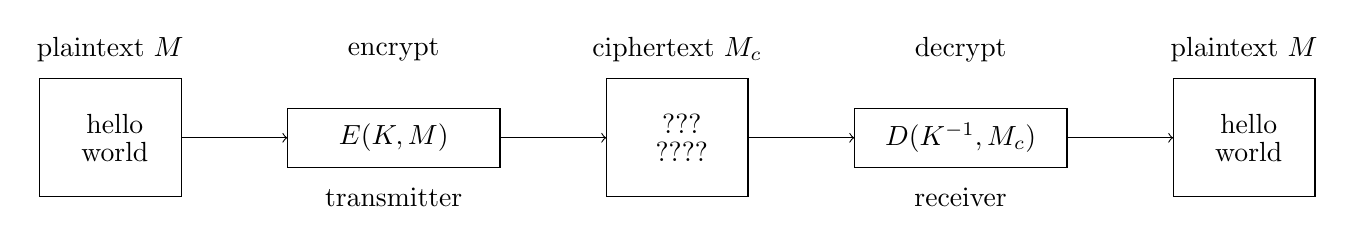
\begin{tikzpicture}[y=0.75cm, x=0.9cm]
                        \begin{scope}[shift={(0, 0)}]
                            \node at (1, 0.5) {plaintext $M$};
                            \node at (1, -1) {\shortstack{~hello~\\~world~}};
                            \draw (0, 0) -- (2, 0) -- (2, -2) -- (0, -2) -- cycle;
                        \end{scope}
                        \begin{scope}[shift={(3.5, 0)}]
                            \node at (1.5, 0.5) {encrypt};
                            \node at (1.5, -2) {transmitter};
                            \node at (1.5, -1) {$E(K, M)$};
                            \draw (0, -0.5) -- (3, -0.5) -- (3, -1.5) -- (0, -1.5) -- cycle;
                        \end{scope}
                        \begin{scope}[shift={(8, 0)}]
                            \node at (1, 0.5) {ciphertext $M_c$};
                            \node at (1, -1) {\shortstack{~???~\\~????~}};
                            \draw (0, 0) -- (2, 0) -- (2, -2) -- (0, -2) -- cycle;
                        \end{scope}
                        \begin{scope}[shift={(11.5, 0)}]
                            \node at (1.5, 0.5) {decrypt};
                            \node at (1.5, -2) {receiver};
                            \node at (1.5, -1) {$D(K^{-1}, M_c)$};
                            \draw (0, -0.5) -- (3, -0.5) -- (3, -1.5) -- (0, -1.5) -- cycle;
                        \end{scope}
                        \begin{scope}[shift={(16, 0)}]
                            \node at (1, 0.5) {plaintext $M$};
                            \node at (1, -1) {\shortstack{~hello~\\~world~}};
                            \draw (0, 0) -- (2, 0) -- (2, -2) -- (0, -2) -- cycle;
                        \end{scope}
                        \draw
                        (2, -1) edge[->] (3.5, -1)
                        (6.5, -1) edge[->] (8, -1)
                        (10, -1) edge[->] (11.5, -1)
                        (14.5, -1) edge[->] (16, -1);
                    \end{tikzpicture}
                \end{center}
                Only certain users should have $K$ (the encryption key), and $K^{-1}$ (the decryption key).
                If someone were to intercept $M_c$, without $K^{-1}$, the attacker can only find $M$ by enumerating all possible $K^{-1}$ via a brute-force attack.
                Another property is that it should be difficult to obtain the values of $K$ and $K^{-1}$ with just $M$ and $M_c$.
                \begin{itemize}
                    \itemsep0em
                    \item secret key (symmetric) encryption has $K = K^{-1}$, hence the same key is used to encrypt and decrypt the file, thus the key must be very carefully distributed otherwise all files can be decrypted
                    \item public key (asymmetric / public-private key pair) encryption has $K \neq K^{-1}$
                        \medskip

                        $K_t$ is the private-key of host $H_t$, and is only stored / used by that host.
                        On the other hand, $K_t^{-1}$ is the public-key of the same host, and is freely distributed.
                        Therefore anything encrypted with $K_t^{-1}$ can only be decrypted by the host $H_t$.
                        This also means anyone can decrypt something encrypted by $H_t$ with $K_t$ - if it is successful, it authenticates the message as coming from $H_t$.
                        \medskip

                        In this example, let $H_t$ have its own private key $K_t$, as well as $H_r$'s public key $K_r^{-1}$ (and vice versa for $H_r$).
                        $H_t$ first signs the message with its own private key, $E(K_t, M)$.
                        It then encrypts the message with the destination's public key, $E(K_r^{-1}, E(K_t, M))$ - ensuring only $H_r$ can read the message.
                        Now, \textbf{only} $H_r$ can obtain the signed message as follows;
                        \begin{center}
                            $D(K_r, E(K_r^{-1}, E(K_t, M))) = E(K_t, M)$
                        \end{center}
                        Additionally, we can validate that the sender was actually $H_t$ with $H_t$'s public key $K_t^{-1}$;
                        \begin{center}
                            $D(K_t^{-1}, E(K_t, M)) = M$
                        \end{center}
                \end{itemize}
                We can compare the two approaches as follows;
                \begin{center}
                    \begin{minipage}[t]{0.485\textwidth}
                        public key (asymmetric)
                        \begin{enumerate}[1.]
                            \itemsep0em
                            \item owner of private-key does not need to disclose its value to communicate
                            \item more secure
                            \item slow encryption / decryption
                            \item example: RSA
                        \end{enumerate}
                    \end{minipage}
                    \hfill
                    \begin{minipage}[t]{0.485\textwidth}
                        secret key (symmetric)
                        \begin{enumerate}[1.]
                            \itemsep0em
                            \item owner of private-key needs to disclose its value in order to communicate
                            \item less secure
                            \item faster encryption / decryption
                            \item example: AES
                        \end{enumerate}
                    \end{minipage}
                \end{center}
            \subsubsection*{Diffie-Hellman Key Exchange}
                An approach for this, to establish a new key on the spot, is the \textit{Diffie-Hellman key exchange}, which can then be used for encryption by symmetric algorithms.
                This can potentially be defeated by powerful systems, but is still used by TLS (formally SSL).
                The (simplified) algorithm is as follows;
                \begin{enumerate}[1.]
                    \itemsep0em
                    \item Bob and Alice agree on a public value $g$ (generator), and a large prime number $p$
                    \item Bob chooses a secret value $b$, and Alice chooses a secret value $a$ (these are not shared) - both values must be lower than $p$
                    \item The secret values are used to calculate their public values (which are then exchanged);
                        \begin{itemize}
                            \itemsep0em
                            \item bob: $x = g^b ~ mod ~ p$
                            \item alice: $y = g^a ~ mod ~ p$
                        \end{itemize}
                    \item They use each other's public value to calculate the \violet{shared secret key} - which can be used to communicate securely;
                        \begin{itemize}
                            \itemsep0em
                            \item bob: $y^b ~ mod ~ p = (g^a ~ mod ~ p)^b ~ mod ~ p \equiv \violet{g^{ab} ~ mod ~ p}$
                            \item alice: $x^a ~ mod ~ p = (g^b ~ mod ~ p)^a ~ mod ~ p \equiv \violet{g^{ab} ~ mod ~ p}$
                        \end{itemize}
                    \item Eve, the eavesdropper, cannot guess / derive the shared secret key, even if they have access to $g, p, x, y$ - since they don't know either of the secret values.
                \end{enumerate}
                An example of this is as follows;
                \begin{align*}
                    a & = 4 \\
                    b & = 5 \\
                    g & = 6 \\
                    p & = p \\
                    \text{(Bob) } x & = (g^b ~ mod ~ p) \\
                    & = 6^5 ~ mod ~ 97 \\
                    & = 7776 ~ mod ~ 97 \\
                    & = 16 \\
                    \text{(Alice) } y & = (g^a ~ mod ~ p) \\
                    & = 6^4 ~ mod ~ 97 \\
                    & = 1296 ~ mod ~ 97 \\
                    & = 35 \\
                    \text{(Bob) } y^b ~ mod ~ p & = 35^5 ~ mod ~ 97 \\
                    & = 52521875 ~ mod ~ 97 \\
                    & = 61 \\
                    \text{(Alice) } x^a ~ mod ~ p & = 16^4 ~ mod ~ 97 \\
                    & = 65536 ~ mod ~ 97 \\
                    & = 61
                \end{align*}
            \subsubsection*{Key Server (Kerberos)}
                Another approach is to have a trusted key server, which the host already knows how to communicate with safely.
                \medskip

                Kerberos (Needham and Schroeder) is a user authentication system which knows your password.
                It also knows the password of the user / resource you want to communicate with.
                It has a KDC (key distribution centre) that can provide tickets, allowing you to communicate with the desired user / resource, which expire after a predefined amount of time.
            \subsubsection*{Hashing}
                When a message is hashed, the original message cannot be retrieved - it one way.
                A hash is a fixed size alphanumeric string, calculated based on a specific input - the hash function should always produce the same hash value with the same input.
                Since it should not be possible to derive the input from the hash value, this can be used for safely storing passwords.
        \subsection*{11th February 2020 \hfill Week 6, Lecture 1}
            The scenario is as follows; an IoT research and design institute will receive government funds for a new device used by the police.
            \begin{itemize}
                \itemsep0em
                \item web servers running Apache 2.4.27 with OpenSSL 1.0.1 on Red Hat Enterprise Linux 7.3
                \item many desktop computers available, running Windows Vista
                    \subitem they are slow, so many staff members bring their own MacBooks to work
                \item reception desk on ground floor, with server room at back of floor secured by RFID card reader
                \item research team on first floor
                \item design team on second floor
                \item HR team shares third floor with CEO and CTO
                \item lower ground level used as storage for technical equipment and parking space
                \item all desktops have wired Ethernet
                    \subitem CEO and CTO have company laptops, wireless AP added on top floor for LAN and Internet connection
                \item employees are planned to be provided with iPads, so they can use iCloud to work from anywhere
                \item installing more access points throughout building
            \end{itemize}
            Some identified security vulnerabilities are as follows;
            \begin{itemize}
                \itemsep0em
                \item server room easily accessible (move to basement)
                \item use biometric scanner instead of RFID
                \item LAN and Internet connected means local network could be exposed
                \item wireless network can be accessed without being in the building (packet sniffing)
                \item sensitive data should not be stored on an external service (iCloud)
                \item OpenSSL 1.0.1 is vulnerable to Heartbleed
                \item Apache 2.4.27 (Optionsbleed) and RHEL 7.3 (Local Privilege Escalation Bug) are all broken (CVE can be easily searched)
                \item Windows Vista
                \item no building security overnight?
                \item employees should not be using personal devices
                \item third-party repairs for MacBooks may expose data
                \item visitor parking area also has technology
                \item insecure connections if working from home (VPN should be used)
                \item employees could be blackmailed or phished (social engineering)
                \item "evil twin" for wireless AP
                \item flood risk for ground floor server room
            \end{itemize}
        \subsection*{13th February 2020 \hfill Week 6, Lecture 2}
            This lecture is the Wireshark practical (enable Promiscuous Mode and Monitor Mode).
            Promiscuous mode works for both wired and wireless connections, and tells the NIC to not drop any packets (for a wireless network; it only focuses on the connected network).
            Monitor mode only works on wireless networks, which tells the NIC to start listening in on all networks - any WiFi network with a password will have encrypted data.
            Most NICs do not support this, or will need different drivers.
            \medskip

            With Wireshark, we can add display filters to the captured packets to select the ones we are interested in, such as;
            \begin{itemize}
                \itemsep0em
                \item ~http.request.method == GET~
                \item ~http contains "password"~
                \item ~ip.src == 192.168.9.220~
            \end{itemize}
        \subsection*{13th February 2020 \hfill Week 6, Lecture 3}
            This continues on from the last lecture, with the Wireshark practical.
            Change the root password for a Raspberry Pi - and ensure new users haven't been created (or keys added).
            \begin{center}
                \textit{"skrrrrr"} - ~root~
            \end{center}
        \subsection*{18th February 2020 \hfill Week 7, Lecture 1}
            \subsubsection*{Introduction to the Network Layer}
                This is also referred to as the Internet Layer, and contains the Internet Protocol (IP).
                At this layer, data travel in IP datagrams (or packets), and data are fragmented into packets, with a layer 3 header added in front of each.
                \medskip

                A router (layer 3) typically has a line in port, which is connected to the ISP via Ethernet, a phone cable, or co-axial.
                There may also additional Ethernet ports to connect devices multiple devices to the local network, via the use of a switch (layer 2) within the router.
                A router is a fundamental component of the network layer (they are the nodes in the graph), and have a finite set of input / output connections.
                It has interfaces (or physical ports - not the same as layer 4 ports), which are individual network interface controllers, and therefore a router can have multiple IP addresses.
            \subsubsection*{Routing}
                The network layer provides facilities to get data from a source to a destination, and may require making many \textbf{hops} at at intermediate routers along the way (frames in the data link layer are moved only within the same network) - this is routing.
                To do this, it must know the topology of the network to choose appropriate paths.
                Load balancing may be used to prevent congestion.
                This layer also has to deal with network heterogeneity, as there may be very old routers still in the network.
            \subsubsection*{Datagram Networks and Forwarding}
                IP is connectionless (each message is routed through the system independent of others, there is also no connection setup or tear-down phase) and packet-switched (each datagram is forwarded from one router to the next based on forwarding decisions).
                This is a best-effort service, with no guarantees on delivery, maximum latency, bandwidth, in-order delivery nor congestion indication.
                \medskip

                There are potentially multiple (possibly asymmetric paths) for the same source / destination.
                In forwarding, we have the destination of the datagram as the input, and an output port as the output.
                A simple design for this is a forwarding table.
                \medskip

                Routers must cooperate to find the best routes between all pairs of nodes, and build a sink tree (or approximation) for each node.
                The sink tree of each node does not contain loops, and only contains the optimal routes towards that specific host.
                \medskip

                Some strategies for routing are as follows;
                \begin{itemize}
                    \itemsep0em
                    \item \textbf{shortest path routing}
                        \medskip

                        Shortest Path Routing (SPR) uses Dijkstra's Algorithm (see \textbf{CO150}), where the labels on arcs represent cost.
                        At each step, we select newly reachable node with the lowest cost, and then add that edge to the tree built so far.
                    \item \textbf{flood routing}
                        \medskip

                        In flood routing, an incoming packet is forwarded across every outgoing link (except the original source).
                        We have to avoid too many packets in the network;
                        \begin{itemize}
                            \itemsep0em
                            \item hop counter \hfill discard a packet after it was forwarded across $N$ routers
                            \item forward only once \hfill avoid cycles, requires storing sequence numbers per source address
                            \item flood selectively \hfill only forward in a direction that makes sense
                        \end{itemize}
                        Flooding always chooses the shortest path because all paths are explored in parallel.
                        This only makes sense to do when \textbf{robustness} is needed, such as in the discovery of unknown destinations.
                    \item \textbf{distance vector routing}
                        \medskip

                        The previous protocols are static, meaning they do not take the current network load into account.
                        DVR, or \textit{Bellman-Ford} is a dynamic protocol that does the following;
                        \begin{enumerate}[1.]
                            \itemsep0em
                            \item consider costs that direct neighbours are advertising to get packet to destination
                            \item select neighbour who's advertised cost, added with own cost to get to that neighbour, is lowest
                            \item advertise the new cost to neighbours
                        \end{enumerate}
                        The main idea is expressed by the Bellman-Ford equation;
                        \begin{center}
                            $D_u^\prime[v] = \min\limits_{x \in \text{neighbours}(u)} (c(u, x) + D_x[v])$
                        \end{center}
                        We want to find the cost of the least cost path from $u$ to $v$.
                        This is the minimum sum of the cost between $u$ and $x$, and the least cost path between $x$ and $v$, where $x$ is each direct neighbour of $u$.
                        At the start, if we don't know anything, we can start with flood routing to discover neighbours.
                        \begin{center}
                            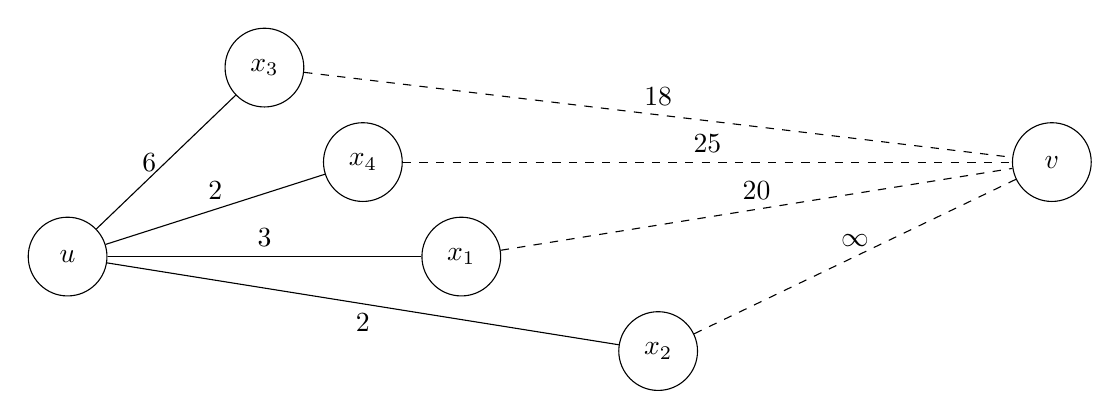
\begin{tikzpicture}[x=2.5cm, y=1.2cm]
                                \node[state, minimum size=1cm] (u) at (-1, 0) {$u$};
                                \node[state, minimum size=1cm] (x1) at (1, -0) {$x_1$};
                                \node[state, minimum size=1cm] (x2) at (2, -1) {$x_2$};
                                \node[state, minimum size=1cm] (x3) at (0, 2) {$x_3$};
                                \node[state, minimum size=1cm] (x4) at (0.5, 1) {$x_4$};
                                \node[state, minimum size=1cm] (v) at (4, 1) {$v$};
                                \draw
                                (u) edge[above] node{3} (x1)
                                (u) edge[below] node{2} (x2)
                                (u) edge[left] node{6} (x3)
                                (u) edge[above] node{2} (x4)
                                (x1) edge[dashed, above] node{20} (v)
                                (x2) edge[dashed, above] node{$\infty$} (v)
                                (x3) edge[dashed, above] node{18} (v)
                                (x4) edge[dashed, above] node{25} (v);
                            \end{tikzpicture}
                        \end{center}
                        An example of this is as follows;
                        \begin{center}
                            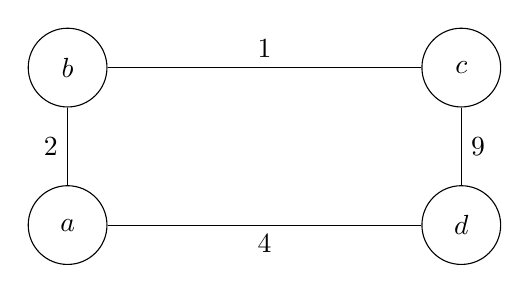
\begin{tikzpicture}[x=5cm, y=2cm]
                                \node[state, minimum size=1cm] (a) at (0, 0) {$a$};
                                \node[state, minimum size=1cm] (b) at (0, 1) {$b$};
                                \node[state, minimum size=1cm] (c) at (1, 1) {$c$};
                                \node[state, minimum size=1cm] (d) at (1, 0) {$d$};
                                \draw
                                (a) edge[below] node{4} (d)
                                (a) edge[left] node{2} (b)
                                (b) edge[above] node{1} (c)
                                (c) edge[right] node{9} (d);
                            \end{tikzpicture}
                        \end{center}
                        \begin{center}
                            \begin{tabular}{|c|cccc|}
                                \hline
                                ($a$) & $a$ & $b$ & $c$ & $d$ \\
                                \hline
                                $D_a$ & 0 & 2 & $\infty$ & 4 \\
                                $D_b$ & $\infty$ & $\infty$ & $\infty$ & $\infty$ \\
                                $D_d$ & $\infty$ & $\infty$ & $\infty$ & $\infty$ \\
                                \hline
                                ($b$) & $a$ & $b$ & $c$ & $d$ \\
                                \hline
                                $D_b$ & 2 & 0 & 1 & $\infty$ \\
                                $D_a$ & $\infty$ & $\infty$ & $\infty$ & $\infty$ \\
                                $D_c$ & $\infty$ & $\infty$ & $\infty$ & $\infty$ \\
                                \hline
                                ($c$) & $a$ & $b$ & $c$ & $d$ \\
                                \hline
                                $D_c$ & $\infty$ & 1 & 0 & 9 \\
                                $D_b$ & $\infty$ & $\infty$ & $\infty$ & $\infty$ \\
                                $D_d$ & $\infty$ & $\infty$ & $\infty$ & $\infty$ \\
                                \hline
                                ($d$) & $a$ & $b$ & $c$ & $d$ \\
                                \hline
                                $D_d$ & 4 & $\infty$ & 9 & 0 \\
                                $D_a$ & $\infty$ & $\infty$ & $\infty$ & $\infty$ \\
                                $D_c$ & $\infty$ & $\infty$ & $\infty$ & $\infty$ \\
                                \hline
                            \end{tabular}
                            \hfill
                            \begin{tabular}{|c|cccc|}
                                \hline
                                ($a$) & $a$ & $b$ & $c$ & $d$ \\
                                \hline
                                $D_a$ & 0 & 2 & \violet{3} & 4 \\
                                $D_b$ & 2 & 0 & 1 & $\infty$ \\
                                $D_d$ & 4 & $\infty$ & 9 & 0 \\
                                \hline
                                ($b$) & $a$ & $b$ & $c$ & $d$ \\
                                \hline
                                $D_b$ & 2 & 0 & 1 & \violet{6} \\
                                $D_a$ & 0 & 2 & $\infty$ & 4 \\
                                $D_c$ & $\infty$ & 1 & 0 & 9 \\
                                \hline
                                ($c$) & $a$ & $b$ & $c$ & $d$ \\
                                \hline
                                $D_c$ & \violet{3} & 1 & 0 & 9 \\
                                $D_b$ & 2 & 0 & 1 & $\infty$ \\
                                $D_d$ & 4 & $\infty$ & 9 & 0 \\
                                \hline
                                ($d$) & $a$ & $b$ & $c$ & $d$ \\
                                \hline
                                $D_d$ & 4 & \violet{6} & 9 & 0 \\
                                $D_a$ & 0 & 2 & $\infty$ & 4 \\
                                $D_c$ & $\infty$ & 1 & 0 & 9 \\
                                \hline
                            \end{tabular}
                            \hfill
                            \begin{tabular}{|c|cccc|}
                                \hline
                                ($a$) & $a$ & $b$ & $c$ & $d$ \\
                                \hline
                                $D_a$ & 0 & 2 & 3 & 4 \\
                                $D_b$ & 2 & 0 & 1 & 6 \\
                                $D_d$ & 4 & 9 & 9 & 0 \\
                                \hline
                                ($b$) & $a$ & $b$ & $c$ & $d$ \\
                                \hline
                                $D_b$ & 2 & 0 & 1 & 6 \\
                                $D_a$ & 0 & 2 & 3 & 4 \\
                                $D_c$ & 3 & 1 & 0 & 9 \\
                                \hline
                                ($c$) & $a$ & $b$ & $c$ & $d$ \\
                                \hline
                                $D_c$ & 3 & 1 & 0 & \violet{7} \\
                                $D_b$ & 2 & 0 & 1 & 6 \\
                                $D_d$ & 4 & 6 & 9 & 0 \\
                                \hline
                                ($d$) & $a$ & $b$ & $c$ & $d$ \\
                                \hline
                                $D_d$ & 4 & 6 & \violet{7} & 0 \\
                                $D_a$ & 0 & 2 & 3 & 4 \\
                                $D_c$ & 3 & 1 & 0 & 9 \\
                                \hline
                            \end{tabular}
                        \end{center}
                        However, there is a problem with DVR - good news propagates quickly, but bad news propagates slowly.
                        Consider the following graph, and assume all costs are 1 (hence we can just look at the number of hops);
                        \begin{center}
                            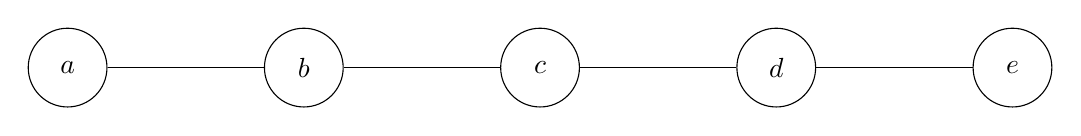
\begin{tikzpicture}[x=1.5cm]
                                \node[state, minimum size=1cm] (a) at (0, 0) {$a$};
                                \node[state, minimum size=1cm] (b) at (2, 0) {$b$};
                                \node[state, minimum size=1cm] (c) at (4, 0) {$c$};
                                \node[state, minimum size=1cm] (d) at (6, 0) {$d$};
                                \node[state, minimum size=1cm] (e) at (8, 0) {$e$};
                                \draw (a) -- (b) -- (c) -- (d) -- (e);
                            \end{tikzpicture}
                        \end{center}
                        Consider the table below, where we have the distance from $a$;
                        \begin{center}
                            \begin{tabular}{|cccc|l|}
                                \hline
                                $b$ & $c$ & $d$ & $e$ & comment \\
                                \hline
                                \hline
                                $\infty$ & $\infty$ & $\infty$ & $\infty$ & initial state \\
                                \hline
                                \multicolumn{5}{|c|}{$a$ comes online after being down} \\
                                \hline
                                1 & $\infty$ & $\infty$ & $\infty$ & after 1 exchange \\
                                1 & 2 & $\infty$ & $\infty$ & after 2 exchanges \\
                                1 & 2 & 3 & $\infty$ & after 3 exchanges \\
                                1 & 2 & 3 & 4 & after 4 exchanges \\
                                \hline
                                \multicolumn{5}{|c|}{$a$ suddenly goes down} \\
                                \hline
                                3 & 2 & 3 & 4 & after 5 exchanges \\
                                3 & 4 & 3 & 4 & after 6 exchanges \\
                                5 & 4 & 5 & 4 & after 7 exchanges \\
                                5 & 6 & 5 & 6 & after 8 exchanges \\
                                7 & 6 & 7 & 6 & after 9 exchanges \\
                                7 & 8 & 7 & 8 & after 10 exchanges \\
                                \hline
                                \multicolumn{5}{|c|}{$\vdots$} \\
                                \hline
                                $\infty$ & $\infty$ & $\infty$ & $\infty$ & \\
                                \hline
                            \end{tabular}
                        \end{center}
                        When $a$ suddenly goes down, they keep increasing their route up to infinity (count-to-infinity problem)
                        We can set infinity to be one more than the longest acceptable path.
                    \item \textbf{link state routing}
                        \medskip

                        This was published in 1979, aiming to replace DVR.
                        The goal is to broadcast information about the network topology to all routers, and each router calculates the sink tree to other routers.
                        Each router does the following;
                        \begin{enumerate}[1.]
                            \itemsep0em
                            \item discover direct neighbours and gets their network addresses
                                \subitem routers know their local network interfaces, and therefore sends a ~HELLO~ packet through each interface - the routers on the other end responds with its address
                            \item calculates cost for sending packet to each neighbour
                                \subitem an ~ECHO~ packet is sent through each interface and the RTT is measured (this gives a reasonable estimate of actual delay)
                            \item constructs LSA (link state advertisement) packet with all information
                                \subitem done with flooding to send LSA to all other routers, once a router has LSAs from every router, it has complete knowledge of the network
                            \item sends that packet to all routers (as well as collecting that packet from all routers) - not limited to just neighbours
                            \item runs Dijkstra's algorithm locally to find shortest paths
                        \end{enumerate}
                        This means that each router stores information about its neighbours, the entire network, and the generated routing table.
                \end{itemize}
                Both DVR and LSR are used, in order to support routers both old (DVR) and new (LSR) routers.
                \begin{center}
                    \begin{tabular}{|l|c|c|}
                        \hline
                        & distance vector routing & link state routing \\
                        \hline
                        network knowledge & local & global \\
                        \hline
                        computation & global & local \\
                        \hline
                        synchronisation & gradual & "instant" (after SPR calculation) \\
                        \hline
                    \end{tabular}
                \end{center}
                These protocols are used internally, and therefore a specific one can be chosen for a local network.
            \subsubsection*{Hierarchical Routing}
                All of the previously discussed routing algorithms require each router to know about the others - this cannot scale, as it becomes too demanding in terms of memory and processing power.
                A solution to this is to introduce regions, and have separate algorithms for intra-region (within the region) and inter-region (between regions) routing.
                Two or three levels is generally sufficient.
                We no longer take an optimal route - we just know where to forward packets.
            \subsubsection*{Broadcast Routing}
                If we want to send a message to (almost) every host on a network, we can take the following approaches;
                \begin{itemize}
                    \itemsep0em
                    \item message each host individually \hfill inefficient
                    \item flood routing \hfill accepted, if we can limit the flood
                    \item multi-destination routing via a list sent with the packet
                        \subitem router checks destination and splits list when forwarding to different interfaces - the message must contain all destinations.
                    \item build sink tree at source and use that for multicast route
                        \subitem must be spanning tree, and routers need to agree on trees
                \end{itemize}
                We can construct this spanning tree with reverse-path forwarding (RPF) broadcast.
                Every router forwards / broadcasts a packet to every adjacent router, except where it came from.
                A router only accepts a broadcast packet $p$ originating at $A$ if $p$ arrives on a link that is on a direct (unicast) path between themselves and $A$.
            \subsubsection*{Multicast Routing}
                We want to send a message to only a subset of nodes, and we need to know when a host enters or leaves a multicast group.
                The solution to this is to construct a spanning tree at each router,  and use a group ID to prune paths that do not contain members of group.
                \medskip

                The main issue with this is scalability - as we need to maintain a spanning tree per source.
                Another approach is to use core-based trees, and have a single spanning tree per group, with the root (core) near the middle of the group.
                For a multicast message to be sent, the host sends it to the core which then performs multicast along the tree.
        \subsection*{20th February 2020 \hfill Week 7, Lecture 2}
            \subsubsection*{Internetworking}
                Internetworking is the process of linking different types of networks together.
                All of these different networks have different protocol stacks, and need to somehow communicate with each other.
                Instead of forcing all networks to run the same stack, we can construct gateways (routers) that interconnect different types of networks.
                Different types of networks include, but are not limited to;
                \begin{itemize}
                    \itemsep0em
                    \item \textbf{PAN} (Personal Area Network) \hfill such as phone connected to PC via Bluetooth (1 user)
                    \item \textbf{LAN} (Local Area Network) \hfill such as laptop connected to desktop via WiFi AP
                    \item \textbf{MAN} (Metropolitan Area Network) \hfill such as displaying bus times without internet (city)
                    \item \textbf{WAN} (Wide Area Network) \hfill such as the Internet
                \end{itemize}
                Additionally, we have the following terminology for devices;
                \begin{itemize}
                    \itemsep0em
                    \item repeaters / hubs \hfill physical layer
                        \subitem boosts signals by repeating everything received at one port to every other port
                    \item switches and bridges \hfill data link layer
                        \subitem creates interconnections by storing a table, and deciding where to forward based on MAC addresses
                    \item multi-protocol routers / gateways \hfill network layer
                        \subitem forwards (and possibly splits up) packets - makes decisions based on IP addresses (note that Transport Layer Gateways and Application Layer Gateways also exist)
                \end{itemize}
            \subsubsection*{The Internet}
                The internet is a collection of autonomous systems (ASes) connected by backbones.
                \medskip

                An application offers a data stream to the transport layer, using either connection-oriented or connection-less services.
                The data stream on the transport layer is converted into an IP datagram for the network layer.
                These are routed through the internet, and routers pass datagrams to the underlying data link layer (LANs and WANs).
                After this, data is in the physical layer, transmitted through cables.
                \medskip

                At the Internet Network Layer, the following needs to be provided;
                \begin{itemize}
                    \itemsep0em
                    \item \textbf{IP} (Internet Protocol)
                        \subitem this includes datagram format, fragmentation, addressing, and packet handling
                    \item \textbf{ICMP} (Internet Control Message Protocol)
                        \subitem this provides error handling, and signalling (such as ~ping~)
                    \item \textbf{DHCP} (Dynamic Host Configuration Protocol)
                        \subitem this provides address configuration
                \end{itemize}
            \subsubsection*{Fragmentation}
                Similar to how TCP includes the sequence number in the header, the layer 3 (IP) header includes the fragment offset from the start of the IP datagram.
                Fragmentation occurs when the router encounters the case where the size of the input datagram exceeds the MTU (maximum transmission unit) of the output link.
                \medskip

                Only the destination reassembles fragmented datagrams, as this pushes complexity out of network.
                Along the path, the datagram may have to be fragmented further.
                The fragmentation scheme must ensure the destination host can figure out if and when all fragments were received, as well as recognising two fragments of the same datagram.
                \medskip

                Assume an initial (non-fragmented) datagram of size $X$.
                The sender assigns a 16-bit identifier to the datagram, and sets the fragment offset (offset in units of 8 bytes) to 0, which indicates this packet contains data starting at position 0 of the original datagram.
                Note that the fragment offset field is 13 bits, hence there can be $2^{13} = 8192$ (0 to 8191) units of 8B in one fragment.
                Note that all fragments should be multiples of 8B, except the last one.
                \medskip

                However, the total length field is 16 bits, therefore it can only support a maximum size of 65535B.
                The IP header itself is 20B, meaning that there are 65515B available, which means that there are 8189 possible units of 8B, and an additional unit of 3B.
                If the more fragments flag is set to 1, more fragments are expected to follow.
                \medskip

                An example of this is as follows - assuming an MTU of 512B, and a total packet size of 1020B;
                \begin{center}
                    \begin{tabular}{cccccc}
                        identifier & fragment offset & more fragments & length & header length & total length \\
                        \hline
                        789 & 0 & 1 & 488 & 20 & 508 \\
                        789 & 61 & 1 & 488 & 20 & 508 \\
                        789 & 122 & 0 & 24 & 20 & 44 \\
                    \end{tabular}
                \end{center}
            \subsubsection*{IPv4 Addressing}
                In IPv4, the addresses are in the format ~XXX.XXX.XXX.XXX~, where ~XXX~ is from 0 to 255 - they are 32-bit, and thus there are 4 billion possible IP addresses.
                Each address is associated with an interface, not host, and therefore a host with multiple interfaces may have more than one IP.
                \medskip

                The key idea is to assign addresses with the same prefix to interfaces belonging to the same organisation.
                Originally, this was done with classful addressing, however this is no longer used as it became apparent that it would quickly run out, due to companies buying more addresses than needed.
                Note in the table below, the leftmost bit is bit 0.
                \begin{center}
                    \begin{tabular}{cccccccc}
                        class & prefix & network bits & max networks & host bits & max hosts & range of host addresses \\
                        \hline
                        \multirow{2}{*}{A} & \multirow{2}{*}{~0~} & \multirow{2}{*}{~1-7~} & \multirow{2}{*}{126} & \multirow{2}{*}{~8-31~} & \multirow{2}{*}{16,777,214} & ~1.0.0.0~ to \\
                        & & & & & & ~127.255.255.255.255~ \\
                        \hline
                        \multirow{2}{*}{B} & \multirow{2}{*}{~10~} & \multirow{2}{*}{~2-15~} & \multirow{2}{*}{16,382} & \multirow{2}{*}{~16-31~} & \multirow{2}{*}{65,536} & ~128.0.0.0~ to \\
                        & & & & & & ~191.255.255.255.255~ \\
                        \hline
                        \multirow{2}{*}{C} & \multirow{2}{*}{~110~} & \multirow{2}{*}{~3-23~} & \multirow{2}{*}{2,097,150} & \multirow{2}{*}{~24-31~} & \multirow{2}{*}{254} & ~192.0.0.0~ to \\
                        & & & & & & ~233.255.255.255.255~ \\
                        \hline
                        \multirow{2}{*}{D} & \multirow{2}{*}{~1110~} & \multicolumn{4}{c}{\multirow{2}{*}{multicast address}} & ~224.0.0.0~ to \\
                        & & & & & & ~239.255.255.255.255~ \\
                        \hline
                        \multirow{2}{*}{E} & \multirow{2}{*}{~1111~} & \multicolumn{4}{c}{\multirow{2}{*}{reserved for future use}} & ~240.0.0.0~ to \\
                        & & & & & & ~255.255.255.255.255~ \\
                        \hline
                    \end{tabular}
                \end{center}
                Nowadays, IP addresses are managed by ICANN to avoid conflicts.
                It delegates parts of address space to regional authorities, which give out IP addresses to ISPs and companies.
            \subsubsection*{Subnet Masking}
                Hosts on the same network must share the same network address.
                The solution to this was to use a single network address for the entire organisation, and divide internally into subnet addresses and host IDs.
                This divides the address into the class, network, subnet, and host, thus introducing a three-level routing hierarchy;
                \begin{enumerate}[1.]
                    \itemsep0em
                    \item external routers only consider the network address, and forward the packet to one of the routers of the organisation
                    \item subnet routers apply the subnet mask, and check if the destination is on their subnet, or if they should forward it to another subnet router
                    \item after host is found, router knows which interface to use to forward packet
                \end{enumerate}
                All interfaces in the same subnet share the same address prefix.
                If we were to get rid of the classes entirely; we will have a notation called classless inter-domain routing (CIDR), which has the format ~address/prefix-length~.
                For example, ~123.1.1.0/24~ means that all addresses share the same leftmost 24 bits with ~123.1.1.0~.
                This scheme is not limited to entire bytes.
                \medskip

                For example; if we were to be asked for the range of addresses in ~128.138.207.160/27~;
                \begin{center}
                    $\overbrace{~10000000 10001010 11001111 101~}^\text{subnet}~00000~$
                    \medskip

                    ~10000000 10001010 11001111 10100000~

                    ~10000000 10001010 11001111 10100001~

                    ~10000000 10001010 11001111 10100010~

                    ~10000000 10001010 11001111 10100011~

                    $\vdots$

                    ~10000000 10001010 11001111 10111110~

                    ~10000000 10001010 11001111 10111111~
                \end{center}
                We would have a range of ~128.138.207.160 - 128.138.207.191~.
                \medskip

                The mask notation is ~address/mask~, and a prefix of length $p$ corresponds to the following mask;
                $$M = \overbrace{~11~ \cdots ~1~}^{p \text{ times}}\underbrace{~00~ \cdots ~0~}_{32 - p \text{ times}}$$
                Therefore we have the following conversions (example);
                \begin{align*}
                    ~128.207.160/27~ & = ~128.207.160/255.255.255.224~ \\
                    ~127.0.0.1/8~ & = ~127.0.0.1/255.0.0.0~ \\
                    ~92.168.0.3/24~ & = ~92.168.0.3/255.255.255.0~ \\
                    ~195.176.181.11/32~ & = ~195.176.181.11/255.255.255.255~
                \end{align*}
                When we (bitwise) ~AND~ the address with the mask, we obtain the network address.
            \subsubsection*{Longest-Prefix Matching}
                Routers attempt to match the maximum possible prefix in order to select the correct network.
                They (bitwise) ~AND~ the IP address with its subnet mask to obtain the network address.
                If they know where this is (based on the router's forwarding table), it will forward it out of the correct port.
                Otherwise, it depends on the algorithm (or a default port where packets for unknown networks go to).
            \subsubsection*{ICMP and NAT}
                ICMP encapsulates control messages in IP packets, and each type is further specified by a code.
                This may be blocked on some routers, as it can be abused, thus a UDP implementation of ~ping~ can be used instead.
                \medskip

                Network Address Translation (NAT) partially solves address shortage by assigning each company a single IP.
                This also allows for home connection to be shared among multiple devices.
                Within a company each device gets a unique local IP used for routing internal traffic, when a packet exits the local network, address translation takes place.
                The following ranges are declared as private to be used in local networks;
                \begin{center}
                    \begin{tabular}{rl}
                        ~10.0.0.0-10.255.255.255/8~ & 16,777,216 addresses \\
                        ~172.16.0.0-172.31.255.255/12~ & 1,048,576 addresses \\
                        ~192.168.0.0-192.168.255.255/16~ & 65,536 addresses
                    \end{tabular}
                \end{center}
                NAT hides the local addresses in the intranet from the public addresses in the internet.
                Other special addresses include the following;
                \begin{itemize}
                    \itemsep0em
                    \item ~0.0.0.0/0~ \hfill default route, used for packet forwarding when no other applicable IP matches
                    \item ~0.0.0.0/8~ \hfill this host on the network (not sent)
                    \item ~127.0.0.0/8~ \hfill loopback (this host, again) but can be sent (~localhost = 127.0.0.1~)
                    \item ~169.254.0.0/16~ \hfill link local (something went wrong trying to acquire an IP address)
                \end{itemize}
                The use of NAT allows one IP to be rented, and then many internal IPs can then be allocated.
                \medskip

                For example, if a connection is set up from ~10.0.0.1~ (local address), on port ~X~, the router uses its public source address ~138.76.29.7~ on port ~Y~, and also registers a mapping $~X~ \leftrightarrow ~Y~$.
                A reply sent to the router on port ~Y~ is then sent to ~10.0.0.1~ on port ~X~.
                \medskip

                Similarly, to allow for incoming connections, port forwarding can be done.
                This is a static mapping on the router, such as telling it to redirect all traffic on port 80 to ~10.0.0.2~ on port 8080.
                \medskip

                While NAT has widespread use, it has a number of problems, and criticism;
                \begin{itemize}
                    \itemsep0em
                    \item violates architectural IP modal, which states an IP address should \textbf{uniquely} identify a single machine worldwide
                    \item changes Internet from connectionless to connection-oriented network (NAT gateway maintains mapping for each connection)
                    \item violates rule of protocol layering by making assumptions about higher layers
                    \item cannot easily support new transport protocols
                    \item P2P protocols may require full connectivity - users behind NAT cannot be contacted directly by peers
                \end{itemize}
                IPv6 deals with all of this, by having many more addresses.
            \subsubsection*{Dynamic Host Configuration Protocol}
                A host needs to determine its own IP address, and this can be done via DHCP (RFC 2131 and 2132);
                \begin{enumerate}[1.]
                    \itemsep0em
                    \item each newly-booted machine broadcasts a ~DHCPDISCOVER~ packet when it connects
                    \item DHCP server (may be the router) replies with the assigned IP address
                        \subitem may maintain static mappings, or assign different addresses each time the host connects
                \end{enumerate}
                To prevent a host from keeping an address for ever, periodic refreshing is required (leasing).
                This is used for a router to receive an IP from the ISP.
        \subsection*{20th February 2020 \hfill Week 7, Lecture 3}
            \subsubsection*{Subnetting Calculations}
                Note that the first address in the subnet (the network address) cannot be assigned to a host.
                Additionally, the last IP address of the subnet is the broadcast address, and also cannot be used for a host.
                The first host address is typically assigned to the router (gateway), but some routers may take the last host address instead.
                \medskip

                For example, with a IP address of ~192.168.1.100~, and a subnet mask of ~255.255.255.0~ (CIDR ~/24~), we have the following addresses;
                \begin{itemize}
                    \itemsep0em
                    \item ~192.168.1.0~ \hfill network address
                    \item ~192.168.1.1~ \hfill first host address (typically the router / gateway)
                    \item ~192.168.1.254~ \hfill last host address (hence 254 host address, out of a total 256 addresses)
                    \item ~192.168.1.255~ \hfill broadcast address
                \end{itemize}
            \subsubsection*{Longest Prefix Matching}
                We have the following routing table;
                \begin{center}
                    \begin{tabular}{c|cc}
                        rule & network & port \\
                        \hline
                        1 & \violet{~123.4~}~.0.0/16~ & 1 \\
                        2 & \violet{~98.7~}~.1.0/16~ & 2 \\
                        3 & \violet{~123.4.20~}~.0/24~ & 2 \\
                        4 & ~(~\violet{~1~}~00...) 128.0.0.0/1~ & 3 \\
                        5 & \violet{~66.249~}~.0.0/16~ & 3 \\
                        6 & ~0.0.0.0/0~ & 4 \\
                        7 & \violet{~128.138~}~.0.0/16~ & 4
                    \end{tabular}
                \end{center}
                Based on the routing table, the following addresses have these output ports;
                \begin{center}
                    \begin{tabular}{cc|l}
                        address & port & comment \\
                        \hline
                        ~123.4.1.69~ & 1 & rule 1 (cannot match the ~20~ on rule 3) \\
                        ~98.7.2.71~ & 2 & rule 2 \\
                        ~200.100.2.1~ & 3 & rule 4 (first bit is a ~1~) \\
                        ~123.4.20.11~ & 2 & rule 3 (can match rule 1, but rule 3 is longer) \\
                        ~123.4.21.10~ & 1 & rule 1 (cannot match the ~20~ on rule 3) \\
                        ~128.138.207.167~ & 4 & rule 7 \\
                        ~68.142.226.44~ & 4 & rule 6 (default route - does not match anything else)
                    \end{tabular}
                \end{center}
            \subsubsection*{Hierarchical Routing}
                A flat network model is too simplistic.
                It doesn't allow for scaling, as transmitting routing information (as well as forwarding) is too expensive.
                Additionally, it has no administrative autonomy, as one organisation may want to run DVR protocol, whereas another may want to run LSR protocol (organisations want different routing protocols), and they also may not want to expose their internal network structures.
                \medskip

                The Internet is organised in Autonomous Systems, which are independent administrative domains, with gateway routers interconnecting autonomous systems.
                There needs to be a distinction between routing within an autonomous system and between autonomous systems;
                \begin{itemize}
                    \itemsep0em
                    \item \textbf{intra-AS routing protocol} \hfill runs within autonomous system
                        \medskip

                        This determines internal routes between any combination of internal routers and gateway routers (in the same AS).
                        This should provide optimal routes, via the use of one of the following;
                        \begin{itemize}
                            \itemsep0em
                            \item \textbf{RIP} (distance vector) \hfill used in old ISPs and small organisations
                            \item \textbf{OSPF - Open Shortest Path First} (link state) \hfill used by larger organisations
                                \medskip

                                This is an abstraction of the network, by collecting the entire network into a directed graph - with the edges representing costs.
                                This then computes the shortest path from every router to every other router.
                                \medskip

                                This allows for ASes on the Internet to be divided into areas.
                                The routers connecting an area to the backbone are referred to as area border routers - responsible for routing packets outside an area.
                                The backbone area routes traffic between other areas in AS.
                        \end{itemize}
                    \item \textbf{inter-AS routing protocol} \hfill determines routing at autonomous-system level
                        \medskip

                        This has to deal with politics, such as some ASes should not be traversed, or are more expensive.
                        \textbf{BGP} (border gateway protocol) is the Internet standard.
                        This is used when traffic is leaving an AS, though the backbone, into another AS.
                        This doesn't care about the best path - just any path.
                        This routing is based on reachability information, as well as policies.
                        It is a path-vector protocol, similar to how DVR announces distances, but instead paths are announced.
                        \medskip

                        Routers advertise routes to networks, with destinations denoted by address prefixes.
                        It may or may not forward an advertisement for a foreign network (as doing so means it is willing to carry traffic for that network).
                        Additionally, prefixes may be aggregated (supernetting) - combining as follows;
                        \begin{align*}
                            \begin{rcases*}
                                ~128.138.242.0/24~ \\
                                ~128.138.243.0/24~
                            \end{rcases*} & \to ~128.138.242.0/23~ \\
                            \\
                            \begin{rcases*}
                                ~192.224.128.0/22~ \\
                                ~192.224.136.0/21~ \\
                                ~192.224.132.0/22~
                            \end{rcases*} & \to ~192.224.128.0/20~
                        \end{align*}
                        The message structure consists of the following;
                        \begin{itemize}
                            \itemsep0em
                            \item ASN (Autonomous System Number) \hfill unique identifier for each AS
                            \item BGP attributes
                                \begin{itemize}
                                    \itemsep0em
                                    \item ~AS-PATH~ \hfill sequence of ASNs through which this advertisement was sent
                                    \item ~NEXT-HOP~
                                        \subitem specifies next interface (IP address) for forwarding packets towards advertised destination (this resolves the cases where the AS is reachable through multiple interfaces)
                                \end{itemize}
                            \item BGP import policy \hfill decides whether to accept or reject route advertisement
                                \subitem router may not want to send traffic through a specific AS listed in ~AS-PATH~
                        \end{itemize}
                        The count-to-infinity problem in DVR is solved with path inspection, where failed routes are spotted and the chosen route can be changed.
                        For example, $F$ receives the following information about the path they take to $D$ from its neighbours;
                        \begin{center}
                            \begin{minipage}[h]{0.3\textwidth}
                                \begin{itemize}
                                    \itemsep0em
                                    \item $B : BCD$
                                    \item $G : GCD$
                                    \item $I : IFGCD$
                                    \item $E : EFGCD$
                                \end{itemize}
                            \end{minipage}
                            \hfill
                            \begin{minipage}[h]{0.55\textwidth}
                                \begin{center}
                                    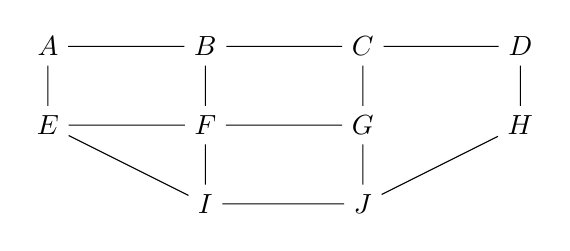
\begin{tikzpicture}[x=2cm]
                                        \node (a) at (0, 0) {$A$};
                                        \node (b) at (1, 0) {$B$};
                                        \node (c) at (2, 0) {$C$};
                                        \node (d) at (3, 0) {$D$};
                                        \node (e) at (0, -1) {$E$};
                                        \node (f) at (1, -1) {$F$};
                                        \node (g) at (2, -1) {$G$};
                                        \node (h) at (3, -1) {$H$};
                                        \node (i) at (1, -2) {$I$};
                                        \node (j) at (2, -2) {$J$};

                                        \draw
                                        (a) -- (b) (a) -- (e)
                                        (b) -- (c) (b) -- (f)
                                        (c) -- (d) (c) -- (g)
                                        (d) -- (h)
                                        (e) -- (f) (e) -- (i)
                                        (f) -- (i) (f) -- (g)
                                        (g) -- (j)
                                        (h) -- (j)
                                        (i) -- (j);
                                    \end{tikzpicture}
                                \end{center}
                            \end{minipage}
                        \end{center}
                        If $G$ crashes, $F$ will see that the routes advertised by $I$ and $E$ fail because they pass through $G$.
                        Therefore $F$ will choose $FBCD$ as its new route.
                        \medskip

                        The routes are ranked according to;
                        \begin{enumerate}[1.]
                            \itemsep0em
                            \item \textbf{preference} value (depends on policy, and can be $\infty$)
                            \item \textbf{shortest} ~AS-PATH~
                            \item \textbf{closest} ~NEXT-HOP~ router
                        \end{enumerate}
                \end{itemize}
                Routers within an AS exchange their intra-AS routing information as expected.
                Gateway routers also discover inter-AS routing information, which is then propagated within AS.
                Both inter-AS and intra-AS routing information is used to populate forwarding tables.
                Destinations within the same AS are reached as usual.
                Destinations outside the AS are reached as follows;
                \begin{itemize}
                    \itemsep0em
                    \item inter-AS information is used to decide is the destination $x$ is reachable through the gateway $G_x$
                    \item intra-AS information is used to decide how to reach $G_x$
                    \item if $x$ is reachable through multiple gateway routers $G_x, G_x^\prime, \dots$, the following strategies can be taken;
                        \begin{itemize}
                            \itemsep0em
                            \item use intra-AS information to determine the costs of paths to $G_x, G_x^\prime, \dots$
                            \item \textbf{hot-potato} routing sends it through the closest gateway
                        \end{itemize}
                \end{itemize}
            \subsubsection*{IPv6}
                The current version if IP cannot support enough addresses, and therefore isn't flexible enough to support many users.
                IPv6 addresses this by supporting billions of hosts, improved security, reducing the size of routing tables, scoped multicasting, and many more improvements.
                It has some backwards compatibility, but adoption is an issue.
                The IPv6 header consists of the following;
                \begin{itemize}
                    \itemsep0em
                    \item version \hfill same as before
                    \item traffic class
                    \item flow label \hfill sets up pseudo-connection between source and destination
                    \item payload length
                    \item next header
                    \item hop limit
                    \item source and destination addresses (128-bit each, also supports anycast address where a single address represents multiple interfaces)
                \end{itemize}
                Fragmentation is pushed onto the end-systems, and the header checksum is no longer used (since TCP and UDP still have checksums).
\end{document}